% !TEX root = main.tex
\section{Decay-time fit}
\label{sec:timeFit}

This section covers the (phase space integrated) decay-time fits to $\Bs\to\Ds\hadron\pion\pion$ data.
We use the \textsf{sFit} technique \cite{Pivk:2004ty} to statistically subtract the background, leaving only the signal PDF to describe the decay-time. 
The \textsf{sWeights} are calculated based on the fit to the reconstructed $B_s$ mass distribution described in Sec.~\ref{sec:massFits}.
The signal PDF is conditional on the tagging decisions $q_i$, the mistag estimates $\eta_i$ ($i=$OS,SS) and the decay-time error $\sigma_t$:
\begin{equation}
\label{eq:TPDF_full}
\mathcal{P}(t \vert \sigma_t, q_{OS}, \eta_{OS}, q_{SS}, \eta_{SS}) \propto \left[ p(t^{'} \vert q_{OS}, \eta_{OS}, q_{SS}, \eta_{SS})  \otimes \mathcal{R}(t - t^{'},\sigma_t) \right] \cdot \epsilon(t)
\end{equation}
where $p(t \vert q_{OS}, \eta_{OS}, q_{SS}, \eta_{SS})$ is given by Equation \ref{eq:PDF_intX} taking the tagging dilution into account.
The decay-time acceptance $\epsilon(t)$ (Sec.~\ref{sec:Acceptance}) and the Gaussian time-resolution function $\mathcal{R}(t - t^{'},\sigma_t)$ (Sec.~\ref{sec:Resolution}) are fixed to the values obtained by the dedicated studies. 
We fix the values of $\Gs$ and $\DGs$ to the latest HFLAV results \cite{HFAG}.

The  unbinned maximum likelihood fits are performed simultaneously in six categories: 
[Run-I,\textsf{L0-TOS}], [Run-I,\textsf{L0-TIS}], %[Run-II,\textsf{L0-TOS}] and [Run-II,\textsf{L0-TIS}].
 [Year-15/16,\textsf{L0-TOS}], [Year-15/16,\textsf{L0-TIS}],
 [Year-17,\textsf{L0-TOS}] and [Year-17,\textsf{L0-TIS}]
 to account for different time-acceptance shapes, time-resolution and tagging calibrations. 
 
 
\subsection{Fit to $\Bs\to\Ds\pion\pion\pion$ data}  
\label{ssec:timeNormFit}

Since the decay $\Bs\to\Ds\pion\pion\pion$ is flavour specific, the \CP coefficients can be fixed to $C=1$ and $D_{f} = D_{\bar{f}} = S_{f} = S_{\bar{f}} = 0$.
The fit determines the calibration parameters for the OS-Combo and SS-Kaon taggers, the $\Bs$ production asymmetry for Run-II data as well as the mixing frequency $\dms$. 
Table \ref{tab:normFitResults} summarizes the fitted parameters. 
The \textsf{sWeighted} decay-time distribution and  the
time-dependent asymmetry $A_{mix}$ between mixed and unmixed $\Bs$ candidates
are shown in Fig.~\ref{fig:tFitNorm} along with the fit projections.

\begin{table}[h]
\centering
\footnotesize
\caption{\small Parameters determined from a fit to the $B_s \to D_s \pi \pi\pi$ decay-time distribution. The uncertainties are statistical and systematic, respectively.}
%\resizebox{\linewidth}{!}{
	\renewcommand{\arraystretch}{1.25}
	\begin{tabular}{l c c c c } 
\hline
\hline
\multicolumn{1}{c}{Decay Channel} & \multicolumn{2}{c}{$A_{b \to c}$} & \multicolumn{2}{c}{$A_{b \to u}$}  \\ 
 & \multicolumn{1}{c}{$\vert a_i \vert$}  & \multicolumn{1}{c}{$arg(a_i) [\degrees]$}  & \multicolumn{1}{c}{$\vert a_i \vert$} & \multicolumn{1}{c}{$arg(a_i) [\degrees]$} \\ 
\hline
 $B_s \to D_s \, ( K_1(1270) \to K \, \rho(770) ) $ &  1.0 & 0.0 & 1.0 & 0.0  \\ 
$\phantom{B_s \to D_s \, (} K_1(1270) \to K^{*}(892) \, \pi \phantom{)} $ & 0.76 $\pm$ 0.11 $\pm$ 0.16 & 60.9 $\pm$ 9.6 $\pm$ 14.0 & &   \\ 
$\phantom{B_s \to D_s \, (} K_1(1270) \to K^{*}_{0}(1430) \, \pi \phantom{)} $ & 0.68 $\pm$ 0.06 $\pm$ 0.34 & 116.5 $\pm$ 5.1 $\pm$ 43.5 & &   \\ 
$B_s \to D_s \, ( K_1(1400) \to K^{*}(892) \, \pi ) $ & 2.53 $\pm$ 0.27 $\pm$ 0.57 & 12.9 $\pm$ 7.4 $\pm$ 8.0 & 0.67 $\pm$ 0.20 $\pm$ 0.51 & -76.3 $\pm$ 16.9 $\pm$ 22.8 \\ 
$B_s \to D_s \, ( K^{*}(1410) \to K^{*}(892) \, \pi ) $ & 1.28 $\pm$ 0.12 $\pm$ 0.24 & 54.9 $\pm$ 5.6 $\pm$ 9.8 &  &  \\ 
$\phantom{B_s \to D_s \, (} K^{*}(1410) \to K \, \rho(770) \phantom{)} $ & 0.66 $\pm$ 0.04 $\pm$ 0.03 & -172.9 $\pm$ 5.0 $\pm$ 6.5 & &   \\ 
$B_s \to D_s \, ( K(1460) \to K^{*}(892) \, \pi ) $ & & &0.77 $\pm$ 0.11 $\pm$ 0.62 & -93.6 $\pm$ 11.2 $\pm$ 12.1 \\ 
$B_s \to ( D_s \, \pi)_{P} \, \, K^{*}(892) $ & 1.02 $\pm$ 0.13 $\pm$ 0.41 & -28.4 $\pm$ 8.0 $\pm$ 10.4 & 0.79 $\pm$ 0.18 $\pm$ 0.35 & 3.7 $\pm$ 12.5 $\pm$ 14.8 \\ 
$B_s \to ( D_s \, K)_{P} \, \, \rho(770) $ & & &0.61 $\pm$ 0.08 $\pm$ 0.26 & 36.4 $\pm$ 7.7 $\pm$ 14.1 \\ 
\hline
\hline
\multicolumn{1}{c}{Fit parameter} & \multicolumn{4}{c}{Value}  \\ 
\hline
\multicolumn{1}{c}{$m_{K_1(1400)} \, [\text{MeV}]$} & \multicolumn{4}{c}{1394.9 $\pm$ 8.8 $\pm$ 12.6 $\pm$ 21.2} \\ 
\multicolumn{1}{c}{$\Gamma_{K_1(1400)} \, [\text{MeV}]$} & \multicolumn{4}{c}{224.0 $\pm$ 15.9 $\pm$ 22.0 $\pm$ 20.9} \\ 
\multicolumn{1}{c}{$m_{K^{*}(1410)} \, [\text{MeV}]$} & \multicolumn{4}{c}{1419.6 $\pm$ 10.8 $\pm$ 26.8 $\pm$ 24.1} \\ 
\multicolumn{1}{c}{$\Gamma_{K^{*}(1410)} \, [\text{MeV}]$} & \multicolumn{4}{c}{342.4 $\pm$ 23.5 $\pm$ 51.0 $\pm$ 52.9} \\ 
 \\ 
\multicolumn{1}{c}{$r$} & \multicolumn{4}{c}{xx.xx $\pm$ 0.04 $\pm$ 0.05 $\pm$ 0.04} \\ 
\multicolumn{1}{c}{$\delta \, [\degrees]$} & \multicolumn{4}{c}{xx.xx $\pm$ 16.1 $\pm$ 6.2 $\pm$ 6.8} \\ 
\multicolumn{1}{c}{$\gamma - 2 \beta_{s} \, [\degrees]$} & \multicolumn{4}{c}{xx.xx $\pm$ 16.1 $\pm$ 11.4 $\pm$ 6.2} \\ 
\hline
\hline
\end{tabular}

%}
\label{tab:normFitResults}
\end{table}

\begin{figure}[h]
	\centering
		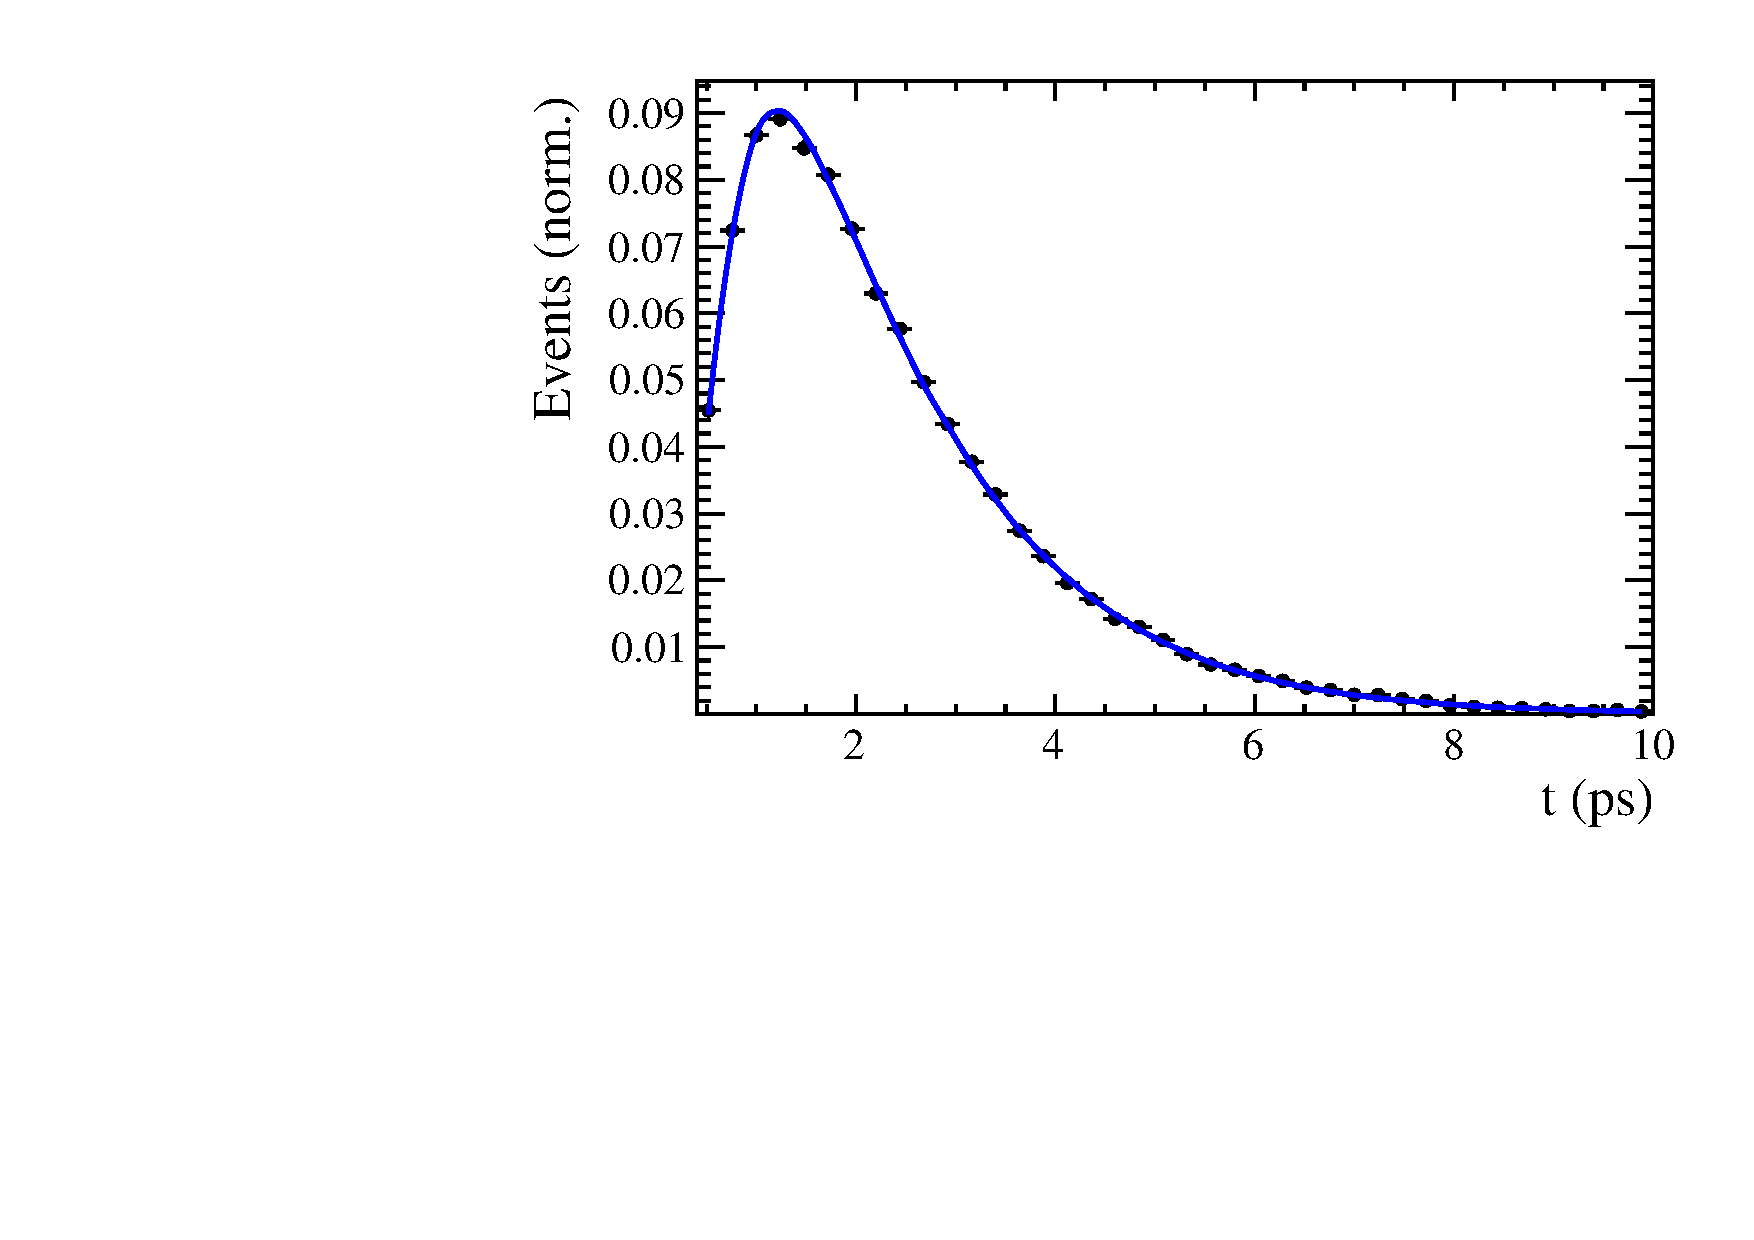
\includegraphics[width=0.4\textwidth, height = !]{figs/timeFit/norm_taggingCalib/h_t.pdf} 
		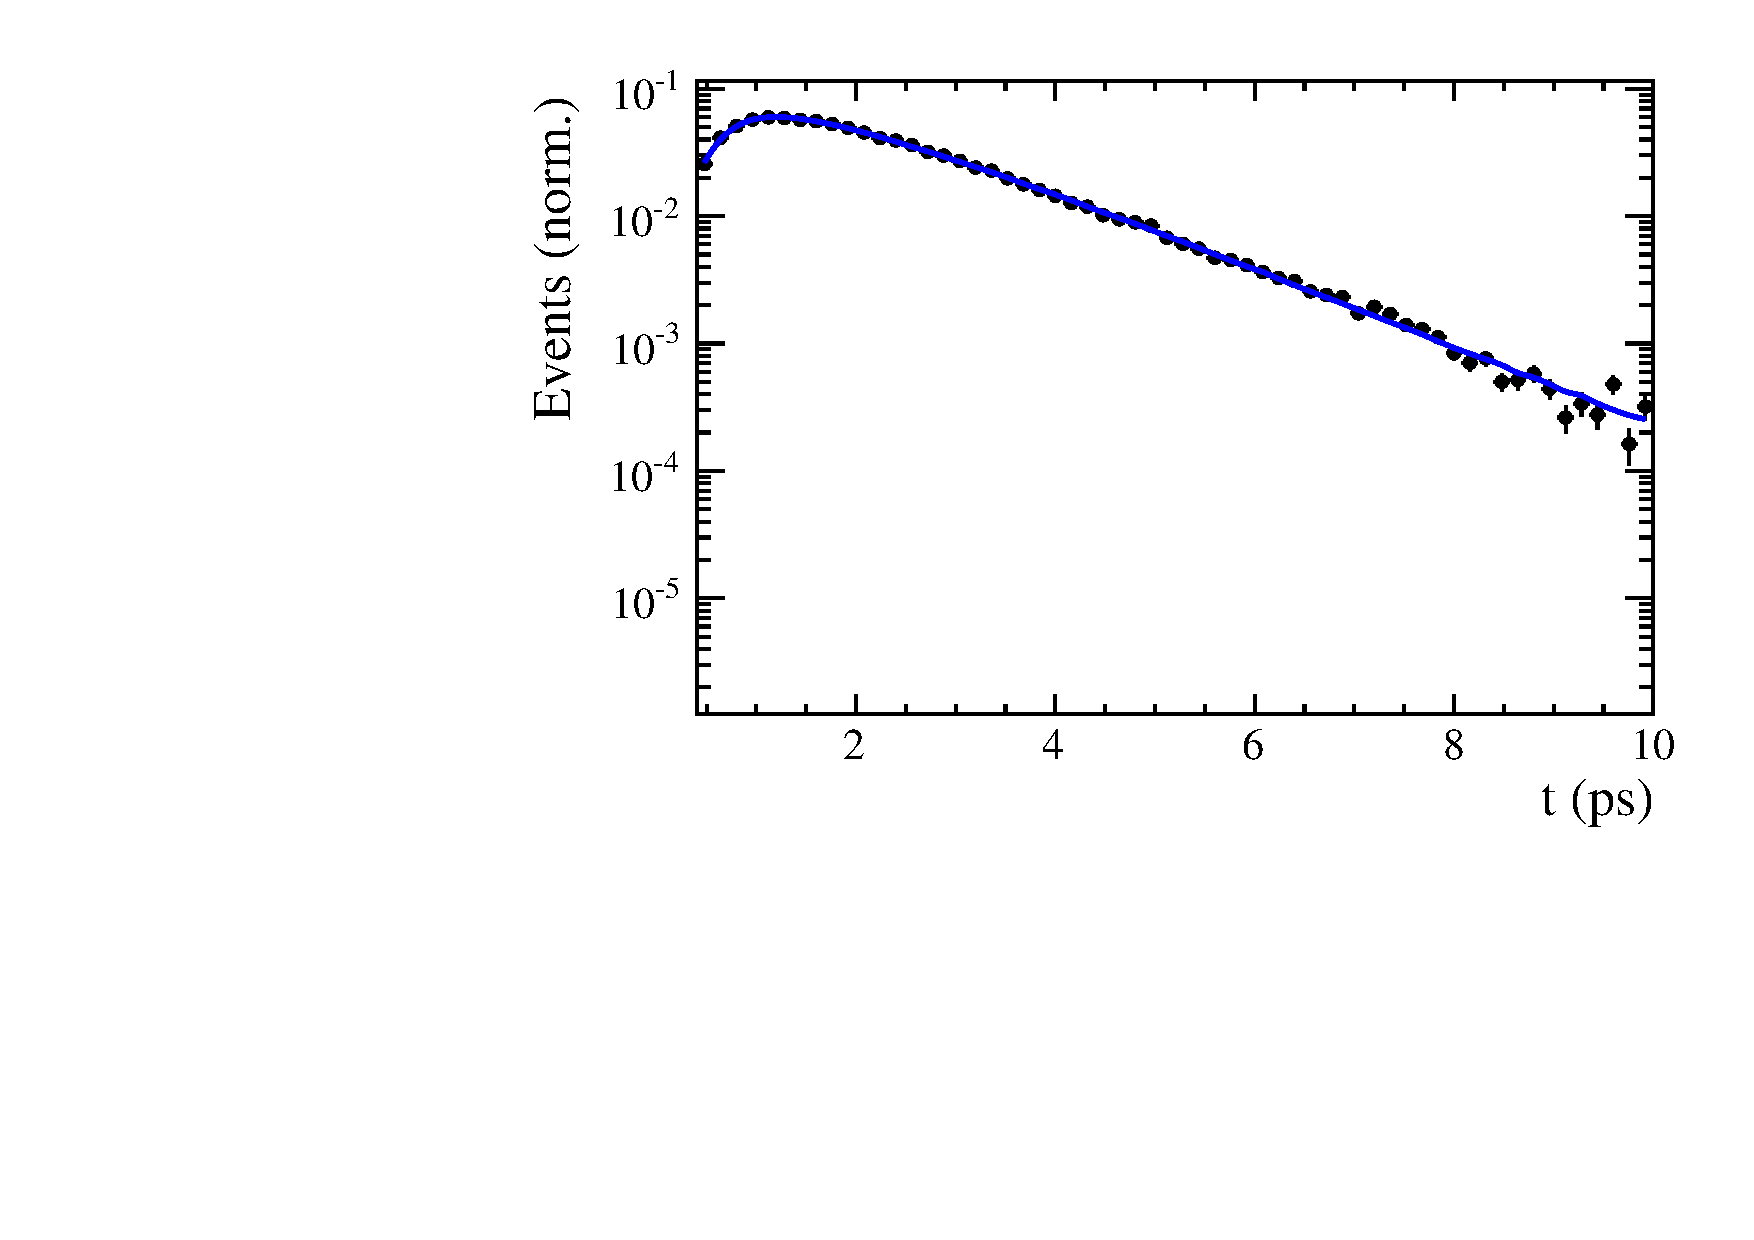
\includegraphics[width=0.4\textwidth, height = !]{figs/timeFit/norm_taggingCalib/h_t_log.pdf} 
		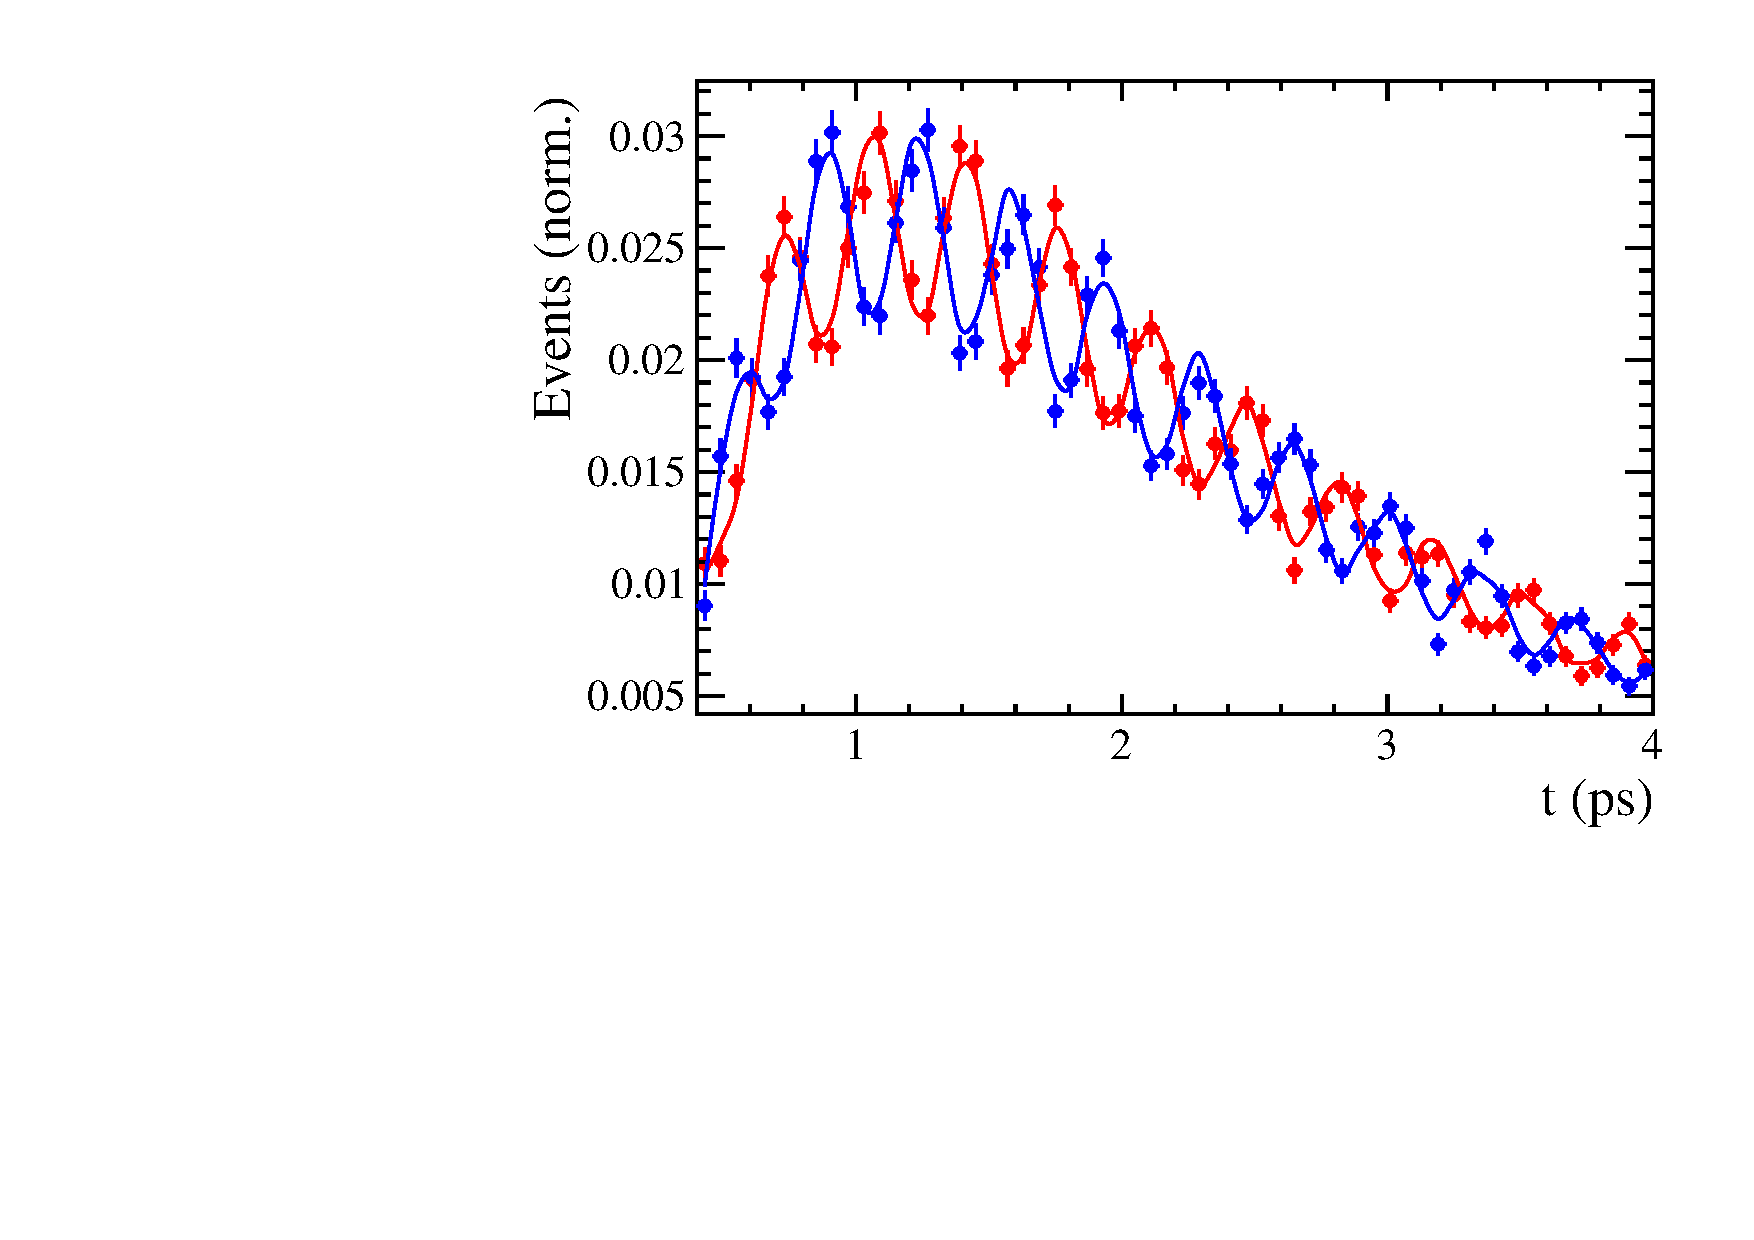
\includegraphics[width=0.4\textwidth, height = !]{figs/timeFit/norm_taggingCalib/h_t_mixed.pdf} 
		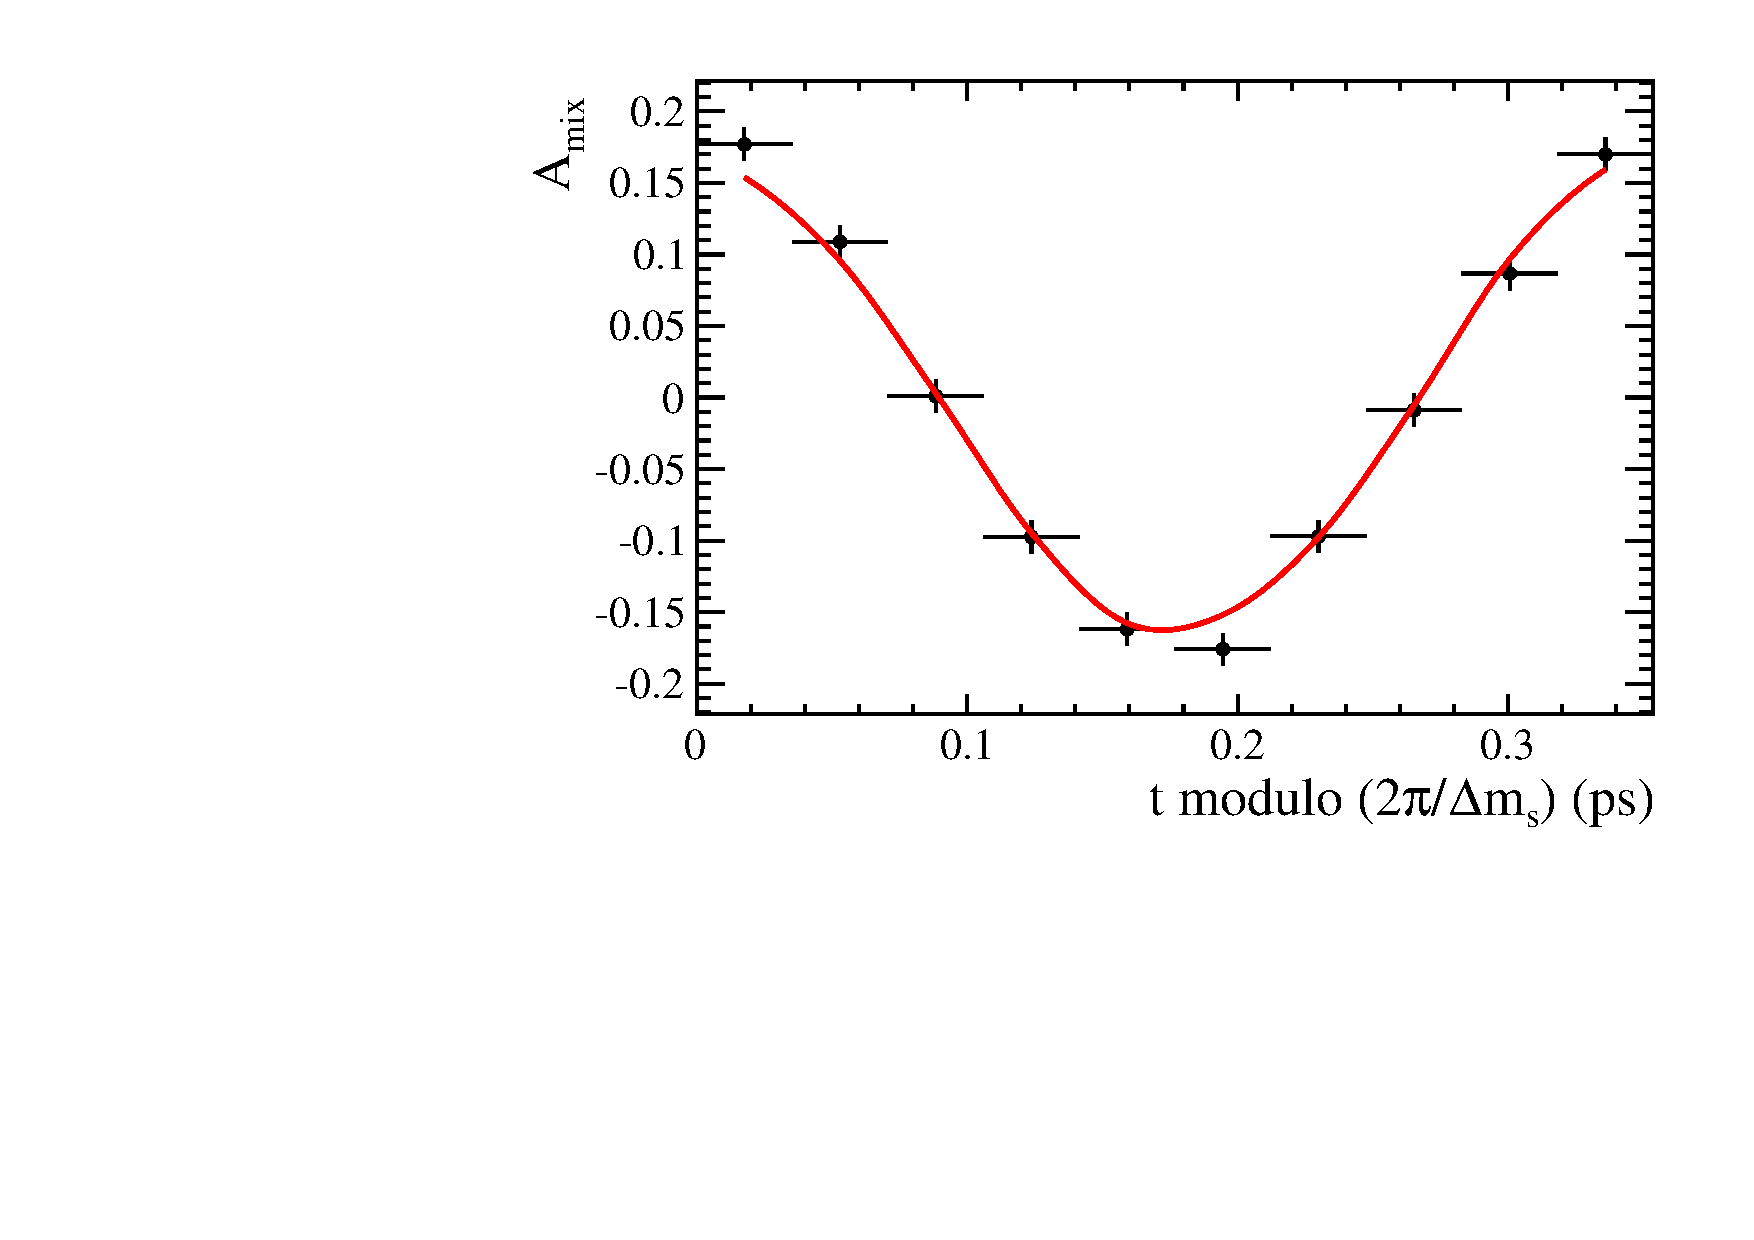
\includegraphics[width=0.4\textwidth, height = !]{figs/timeFit/norm_taggingCalib/h_asym.pdf} 		
		\caption{
		\footnotesize Top: Flavour averaged decay time distribution of $\Bs\to\Ds\pion\pion\pion$ candidates. 
Bottom-left: Tagged decay time distribution of mixed (red) and unmixed (blue) signal candidates. 
Bottom-right: Time-dependent asymmetry $A_{mix}$ between mixed and unmixed $\Bs$ candidates folded into one oscillation period.} 		
		\label{fig:tFitNorm}
\end{figure}	

%\clearpage
\subsection{Fit to $\Bs\to\Ds\kaon\pion\pion$ data}
\label{ssec:timeFit}

%The time-dependent fit to the sWeighted sample of $\Bs\to\Ds\kaon\pion\pion$ signal candidates is performed simultaneously in the four bins defined in Sec. \ref{subsec: AccComparison}, 
%spliting the data into Run I \& II and trigger category 0 (L0Hadron TOS) \& 1 (L0Hadron TIS). 
%In these four bins, the respective description of the decay-time acceptance (Sec. \ref{sec:Acceptance}) is used as an input. 
%As further input the decay-time resolution scaling relation, found separately for Run I \& II in Sec. \ref{sec:Resolution}, is used in the simultaneous fit. 
%The full fit model is given in Eq. \ref{eq:TPDF_full}, where $\int P(x,t,q_t,q_f)$ is: 
%
%\begin{equation} 
%           \int P(x,t,q_t,q_f) \text d x \propto    [
%        \, \text{cosh} \left( \frac{\Delta \Gamma \, t}{2}\right) 
%          + q_t q_f \, C \, \text{cos} \left( m_s \, t \right)  
%          + \kappa \, D_{q_f} \, \text{sinh} \left( \frac{\Delta \Gamma \, t}{2}\right)  
%          - q_t \, \kappa \, S_{q_f}\, \text{sin} \left( m_s \, t \right)  ]  e^{- \Gamma t}.
%\end{equation}
%
%Note that the integration over the available phase space $x$ gives rise to the coherence factor $\kappa$, which dilutes the sensitivity to the CP coefficients $D$ \& $S$ and with that, also to the CKM phase $\gamma$. 
%All input parameters from the tagging, time acceptance and resolution are fixed in the fit. The CP coefficients, as well as $\kappa$, are therefore the only parameters left floating. 

The measured \CP coefficients $C,D_{f},D_{\bar{f}},S_{f} $ and $S_{\bar{f}}$ extracted from a 
fit to the $B_s \to D_s K \pi\pi$ decay-time distribution are reported in Table \ref{tab:sigFitResults}.
The fit projection is shown in Fig.~\ref{fig:tFitSig}.
We included a multi-dimensional Gaussian-constraint for the tagging calibration parameters (including the tagging asymmetries) with the central values and covariance matrix determined in Sec.~\ref{ssec:timeNormFit}.

The \CP coefficients are converted to the observables $r,\kappa,\delta,\gamma$ using the GammaCombo package.
The corresponding confidence levels  are shown in Fig~\ref{fig:FitCL}.
\newline
\\
\pretextcomment{
As the central values of the \CP coefficients are blinded, we calculate naive estimates of them assuming the following values for the physical observables:
$r=0.4, \kappa = 0.5, \delta = 10^\circ, \gamma = 70^\circ$.
We plug the values of the  \CP coefficients obtained in this way, with the correct  uncertainties as extracted from data,  into the GammaCombo tool. 
Note that the uncertainties of the physical observables depend strongly on the central values of the \CP coefficients, so this exercise 
should only be considered as a rough estimated of the expected sensitivity.
 }

%\newline
%\\
\pretextcomment{
Currently the mixing frequency is fixed to the HFLAV value for the fit to $B_s \to D_s K \pi\pi$ data. 
We intend to update the fit after unblinding our result from the $\Bs\to\Ds\pion\pion\pion$ fit since our precision is significantly higher.
}
\begin{figure}[h]
	\centering
		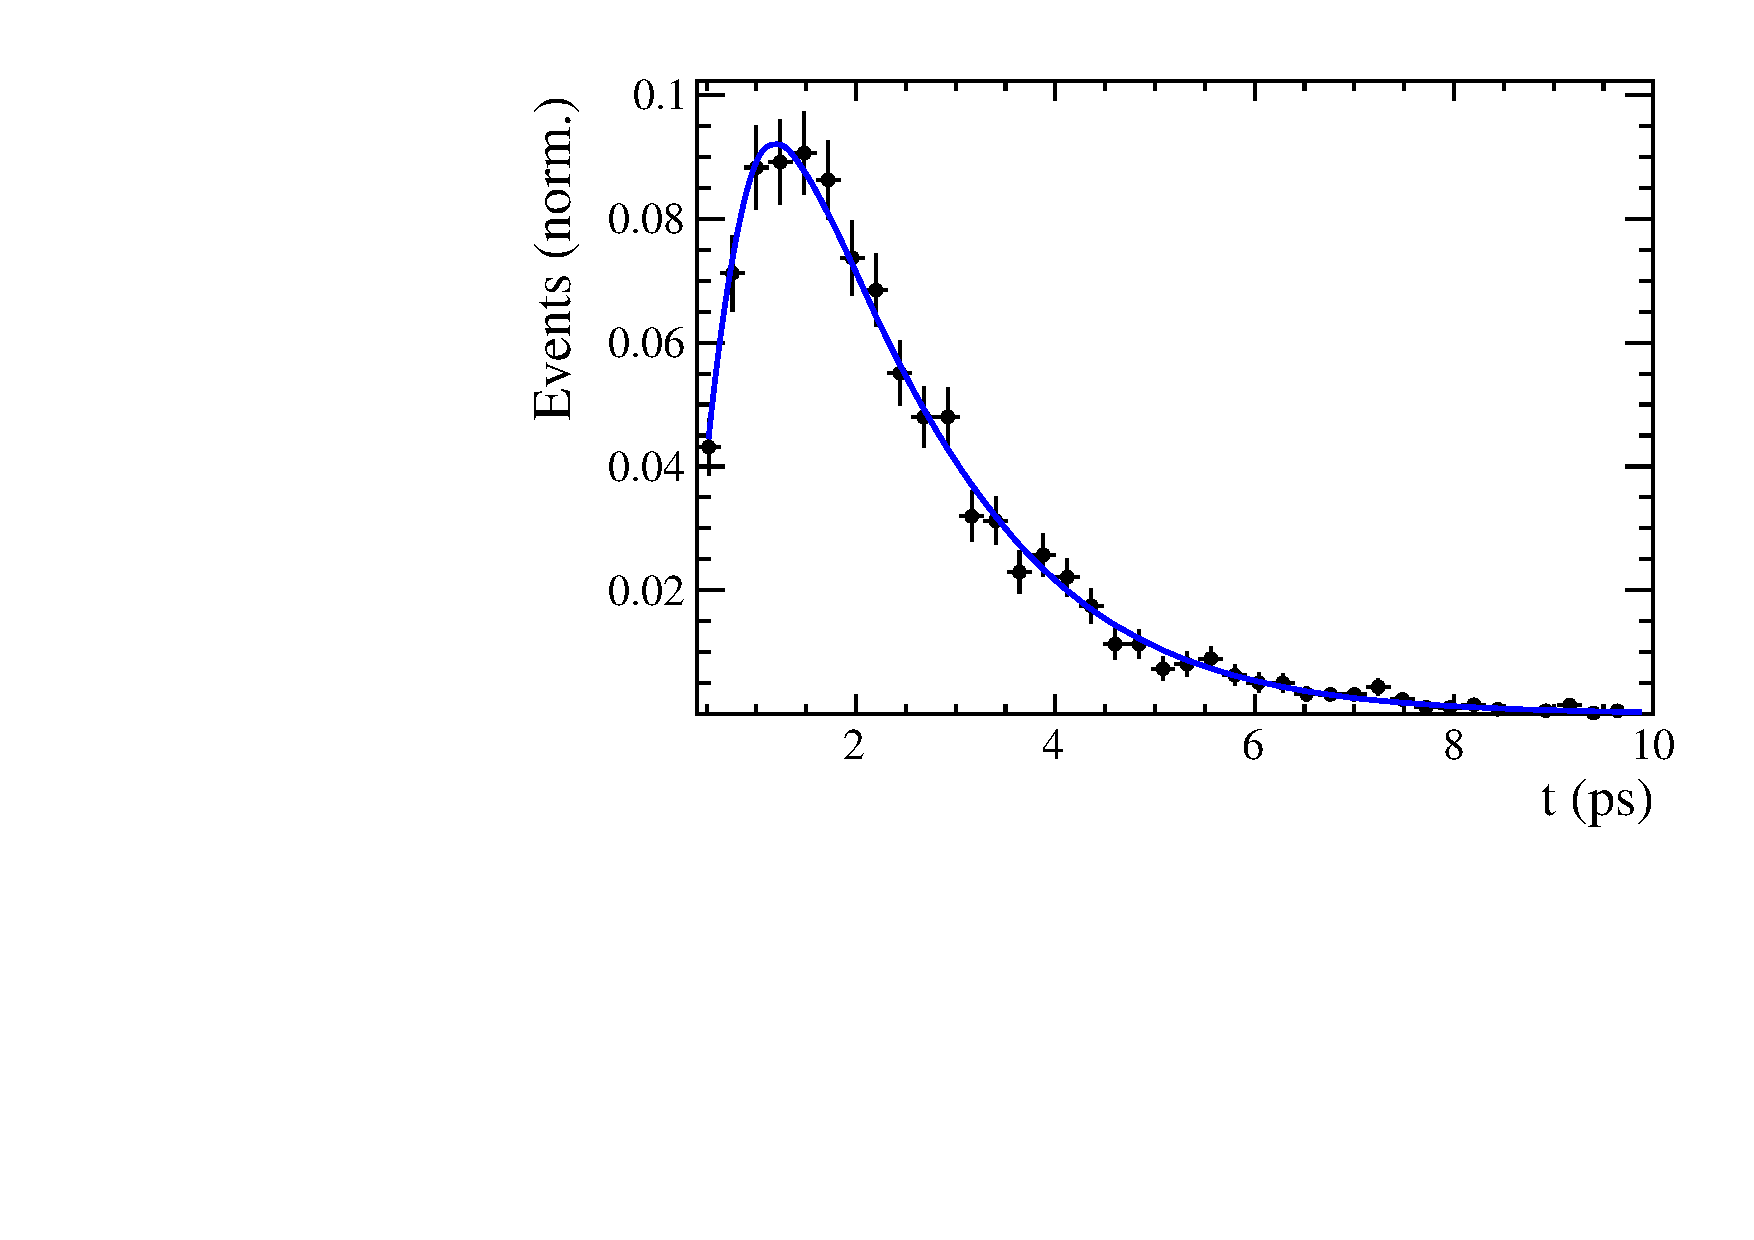
\includegraphics[width=0.4\textwidth, height = !]{figs/timeFit/signal/h_t.pdf} 
		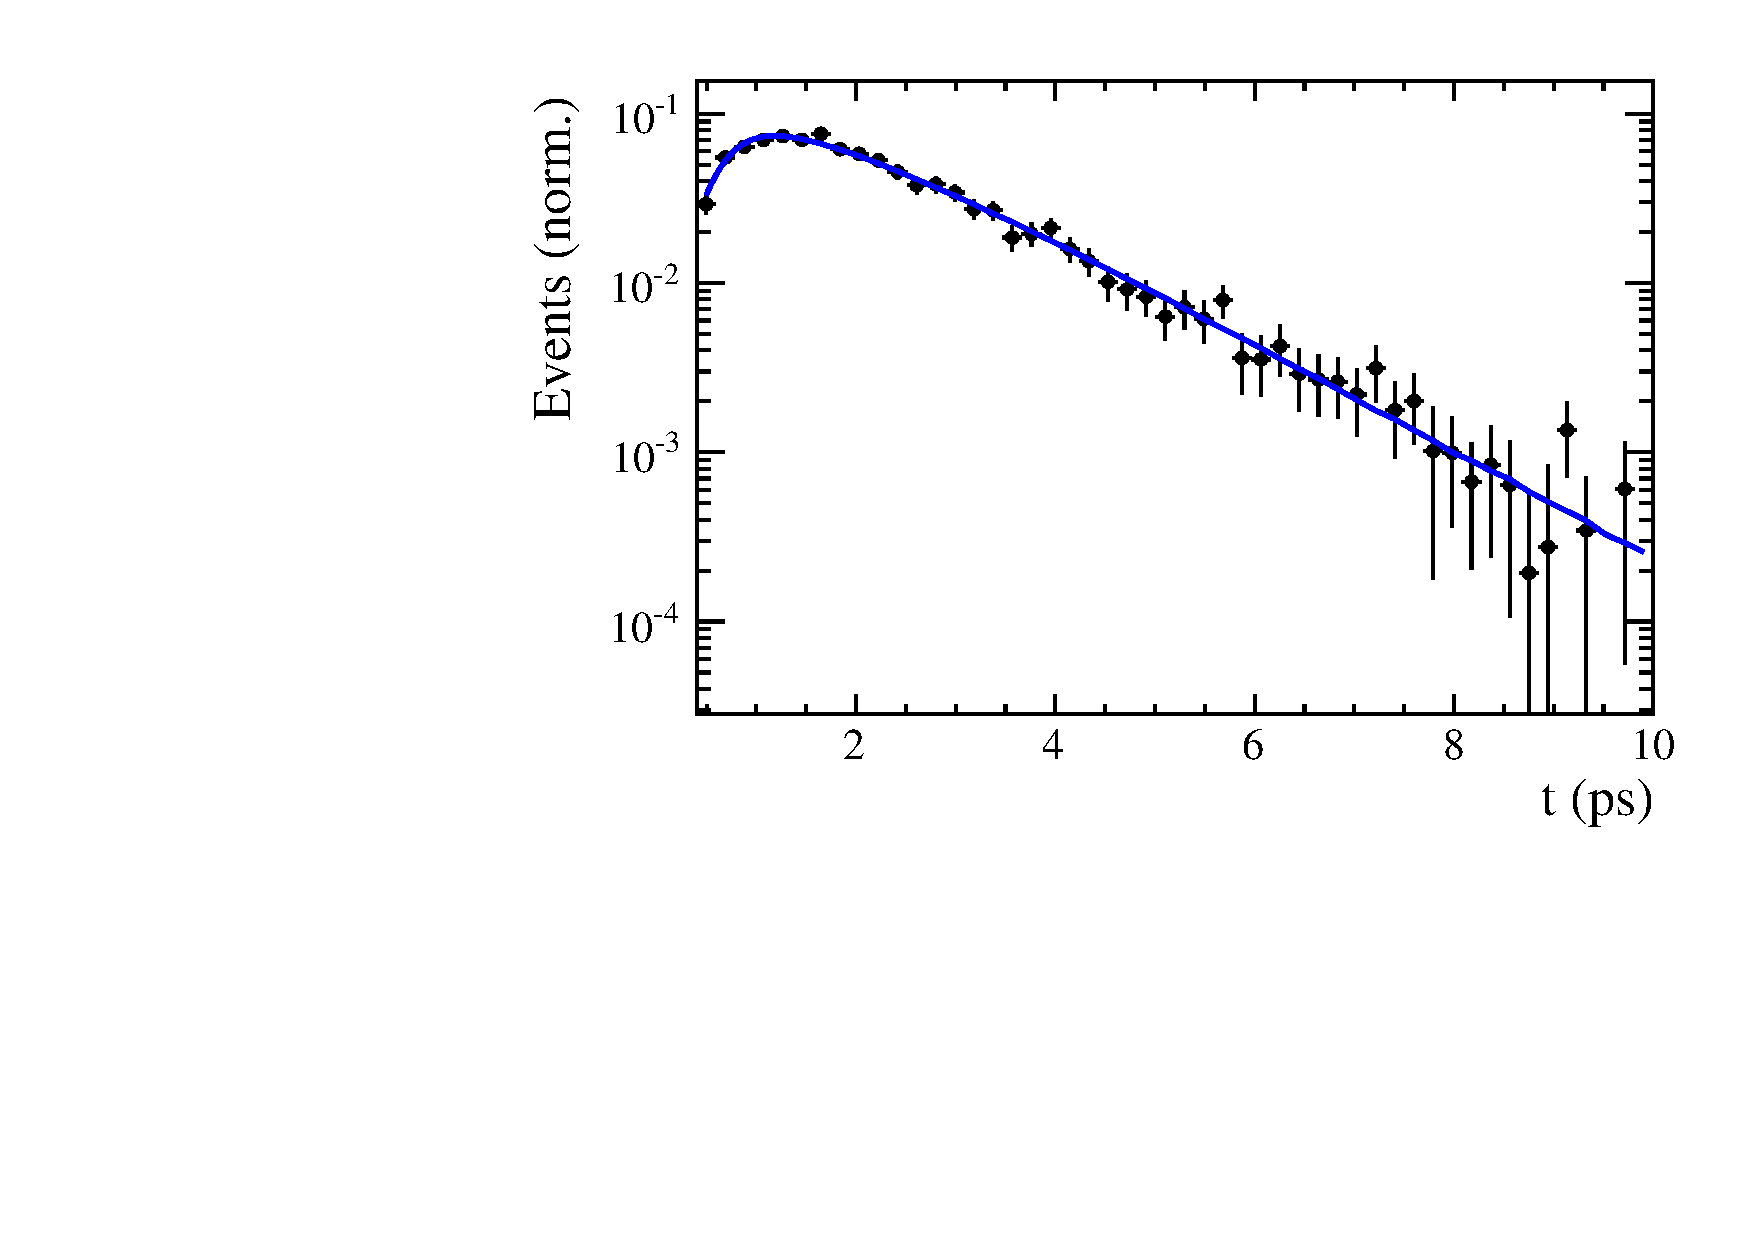
\includegraphics[width=0.4\textwidth, height = !]{figs/timeFit/signal/h_t_log.pdf} 
%		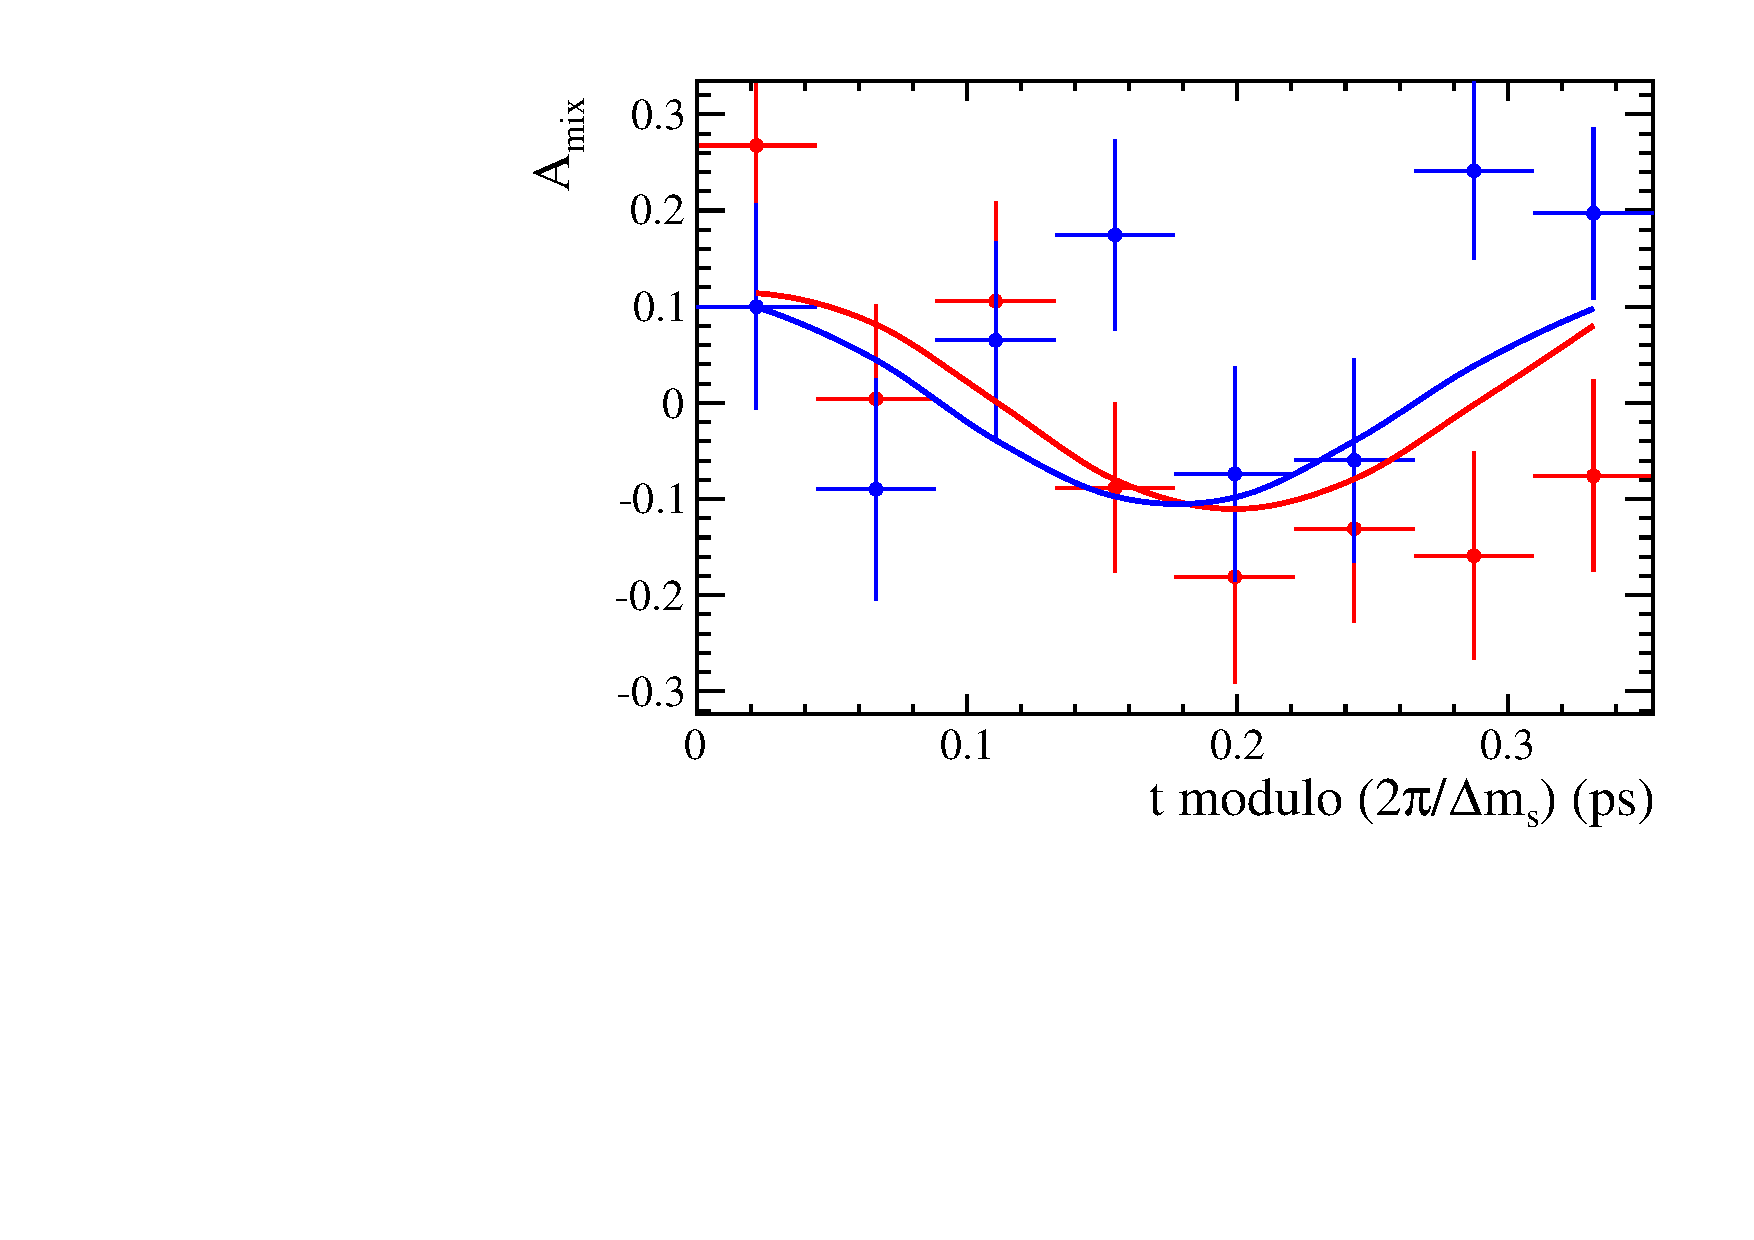
\includegraphics[width=0.45\textwidth, height = !]{figs/timeFit/signal/h_asym.pdf} 		
		\caption{Decay-time distribution of $\Bs\to\Ds\kaon\pion\pion$ signal candidates with the fit projection overlaid.} 
		\label{fig:tFitSig}
\end{figure}	

\begin{table}[h]
\centering
\caption{\CP coefficients determined from a fit to the $B_s \to D_s K \pi\pi$ decay-time distribution. The uncertainties are statistical and systematic, respectively.}
%\resizebox{\linewidth}{!}{
	\renewcommand{\arraystretch}{1.5}
	\begin{tabular}{l c c c c } 
\hline
\hline
\multicolumn{1}{c}{Decay Channel} & \multicolumn{2}{c}{$A_{b \to c}$} & \multicolumn{2}{c}{$A_{b \to u}$}  \\ 
 & \multicolumn{1}{c}{$\vert a_i \vert$}  & \multicolumn{1}{c}{$arg(a_i) [\degrees]$}  & \multicolumn{1}{c}{$\vert a_i \vert$} & \multicolumn{1}{c}{$arg(a_i) [\degrees]$} \\ 
\hline
 $B_s \to D_s \, ( K_1(1270) \to K \, \rho(770) ) $ &  1.0 & 0.0 & 1.0 & 0.0  \\ 
$\phantom{B_s \to D_s \, (} K_1(1270) \to K^{*}(892) \, \pi \phantom{)} $ & 0.76 $\pm$ 0.11 $\pm$ 0.16 & 60.9 $\pm$ 9.6 $\pm$ 14.0 & &   \\ 
$\phantom{B_s \to D_s \, (} K_1(1270) \to K^{*}_{0}(1430) \, \pi \phantom{)} $ & 0.68 $\pm$ 0.06 $\pm$ 0.34 & 116.5 $\pm$ 5.1 $\pm$ 43.5 & &   \\ 
$B_s \to D_s \, ( K_1(1400) \to K^{*}(892) \, \pi ) $ & 2.53 $\pm$ 0.27 $\pm$ 0.57 & 12.9 $\pm$ 7.4 $\pm$ 8.0 & 0.67 $\pm$ 0.20 $\pm$ 0.51 & -76.3 $\pm$ 16.9 $\pm$ 22.8 \\ 
$B_s \to D_s \, ( K^{*}(1410) \to K^{*}(892) \, \pi ) $ & 1.28 $\pm$ 0.12 $\pm$ 0.24 & 54.9 $\pm$ 5.6 $\pm$ 9.8 &  &  \\ 
$\phantom{B_s \to D_s \, (} K^{*}(1410) \to K \, \rho(770) \phantom{)} $ & 0.66 $\pm$ 0.04 $\pm$ 0.03 & -172.9 $\pm$ 5.0 $\pm$ 6.5 & &   \\ 
$B_s \to D_s \, ( K(1460) \to K^{*}(892) \, \pi ) $ & & &0.77 $\pm$ 0.11 $\pm$ 0.62 & -93.6 $\pm$ 11.2 $\pm$ 12.1 \\ 
$B_s \to ( D_s \, \pi)_{P} \, \, K^{*}(892) $ & 1.02 $\pm$ 0.13 $\pm$ 0.41 & -28.4 $\pm$ 8.0 $\pm$ 10.4 & 0.79 $\pm$ 0.18 $\pm$ 0.35 & 3.7 $\pm$ 12.5 $\pm$ 14.8 \\ 
$B_s \to ( D_s \, K)_{P} \, \, \rho(770) $ & & &0.61 $\pm$ 0.08 $\pm$ 0.26 & 36.4 $\pm$ 7.7 $\pm$ 14.1 \\ 
\hline
\hline
\multicolumn{1}{c}{Fit parameter} & \multicolumn{4}{c}{Value}  \\ 
\hline
\multicolumn{1}{c}{$m_{K_1(1400)} \, [\text{MeV}]$} & \multicolumn{4}{c}{1394.9 $\pm$ 8.8 $\pm$ 12.6 $\pm$ 21.2} \\ 
\multicolumn{1}{c}{$\Gamma_{K_1(1400)} \, [\text{MeV}]$} & \multicolumn{4}{c}{224.0 $\pm$ 15.9 $\pm$ 22.0 $\pm$ 20.9} \\ 
\multicolumn{1}{c}{$m_{K^{*}(1410)} \, [\text{MeV}]$} & \multicolumn{4}{c}{1419.6 $\pm$ 10.8 $\pm$ 26.8 $\pm$ 24.1} \\ 
\multicolumn{1}{c}{$\Gamma_{K^{*}(1410)} \, [\text{MeV}]$} & \multicolumn{4}{c}{342.4 $\pm$ 23.5 $\pm$ 51.0 $\pm$ 52.9} \\ 
 \\ 
\multicolumn{1}{c}{$r$} & \multicolumn{4}{c}{xx.xx $\pm$ 0.04 $\pm$ 0.05 $\pm$ 0.04} \\ 
\multicolumn{1}{c}{$\delta \, [\degrees]$} & \multicolumn{4}{c}{xx.xx $\pm$ 16.1 $\pm$ 6.2 $\pm$ 6.8} \\ 
\multicolumn{1}{c}{$\gamma - 2 \beta_{s} \, [\degrees]$} & \multicolumn{4}{c}{xx.xx $\pm$ 16.1 $\pm$ 11.4 $\pm$ 6.2} \\ 
\hline
\hline
\end{tabular}

%}
\label{tab:sigFitResults}
\end{table}


\begin{figure}[h]
	\centering
		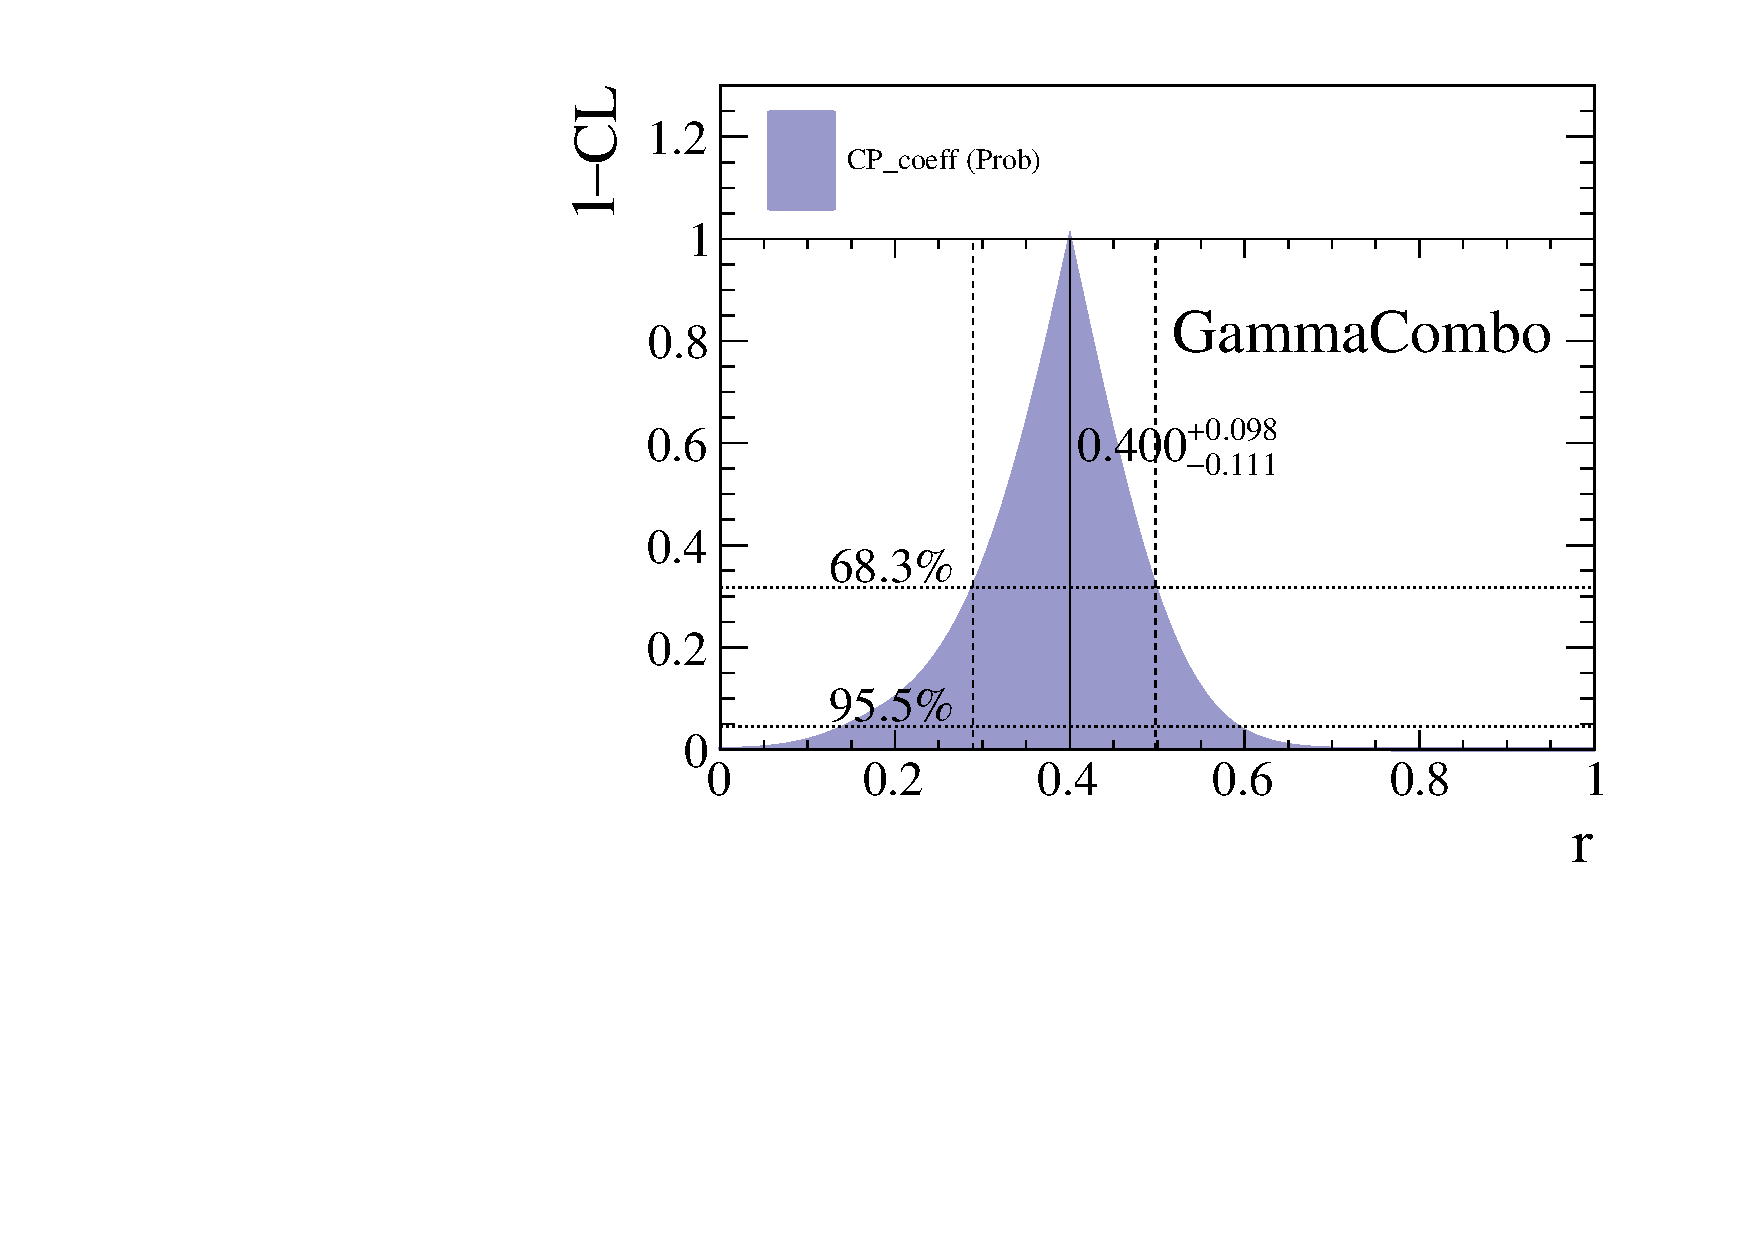
\includegraphics[width=0.4\textwidth, height = !]{figs/GammaCombo/signal_toy/cartesian_cp_coeff_r.pdf} 
		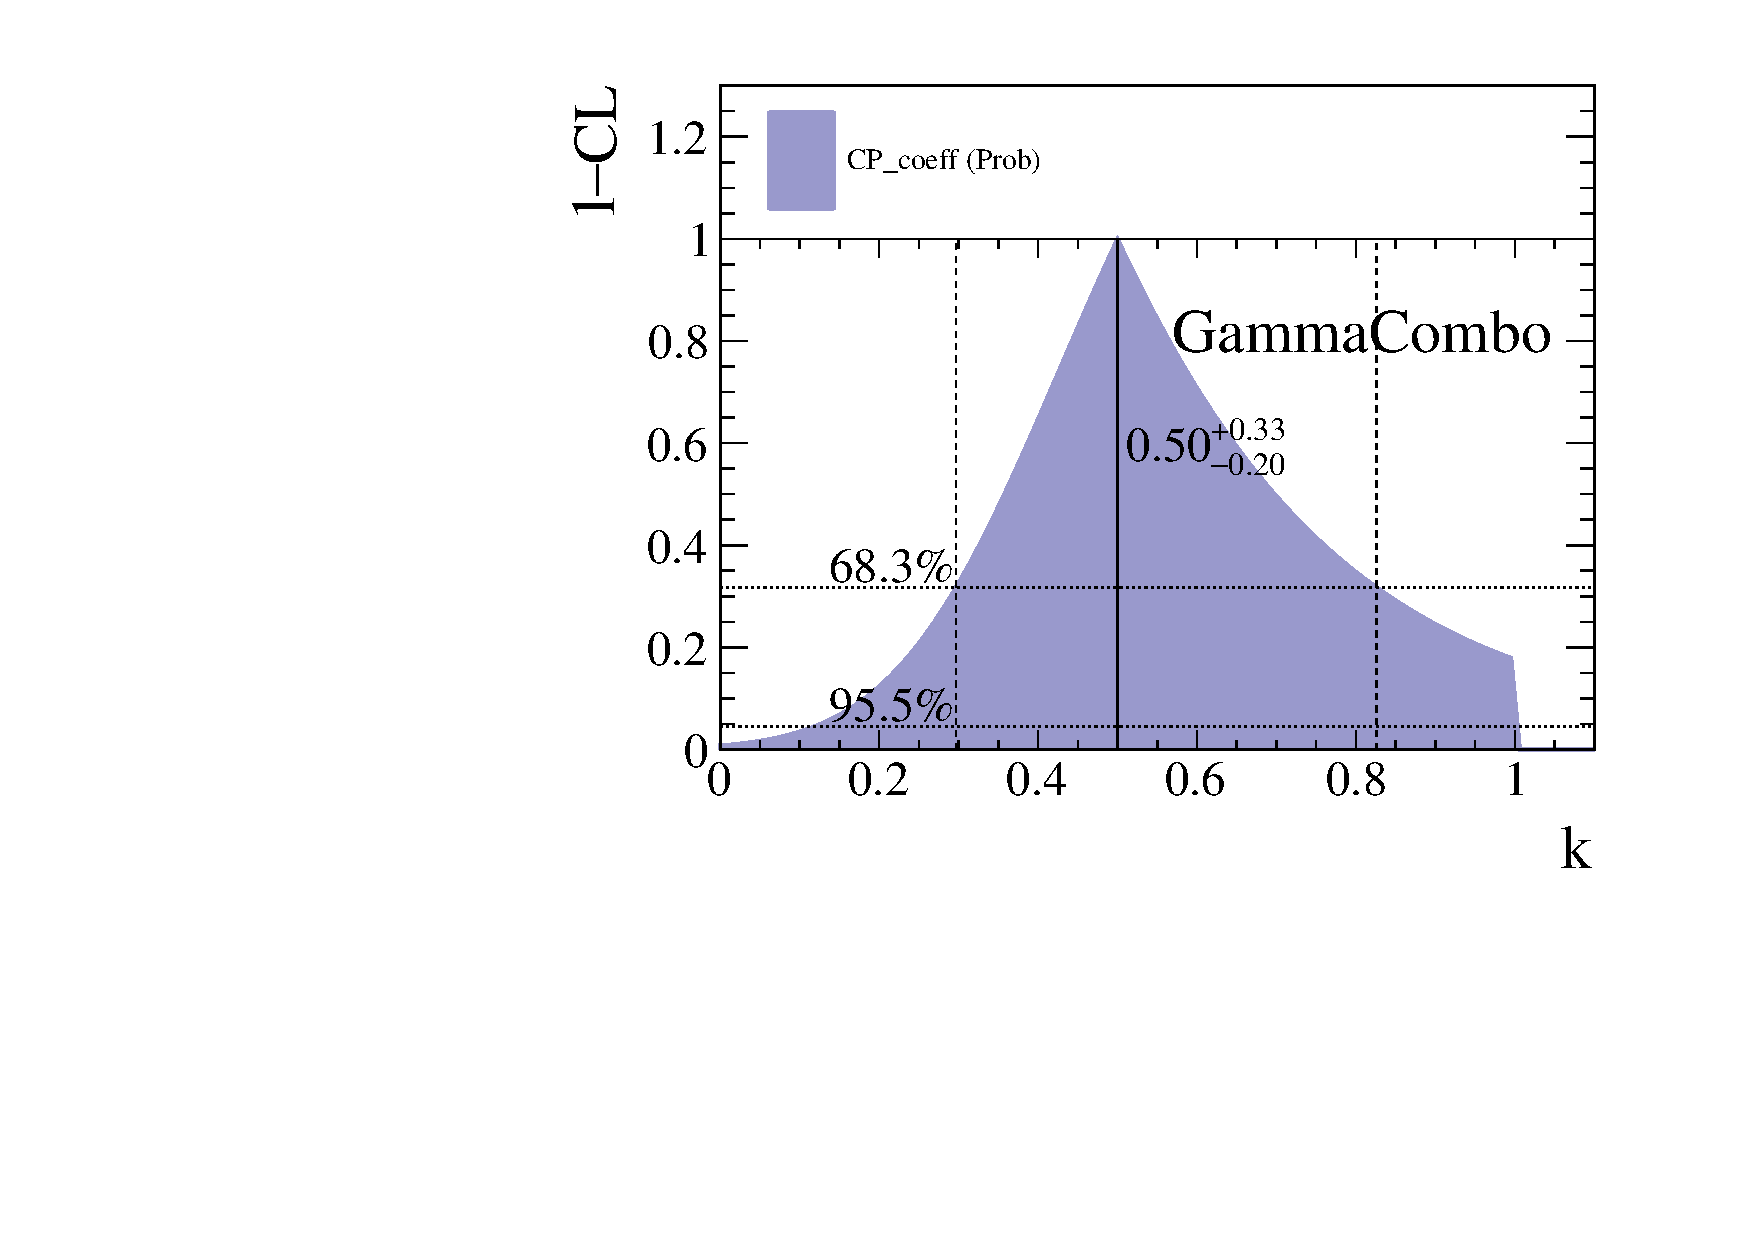
\includegraphics[width=0.4\textwidth, height = !]{figs/GammaCombo/signal_toy/cartesian_cp_coeff_k.pdf} 
		
		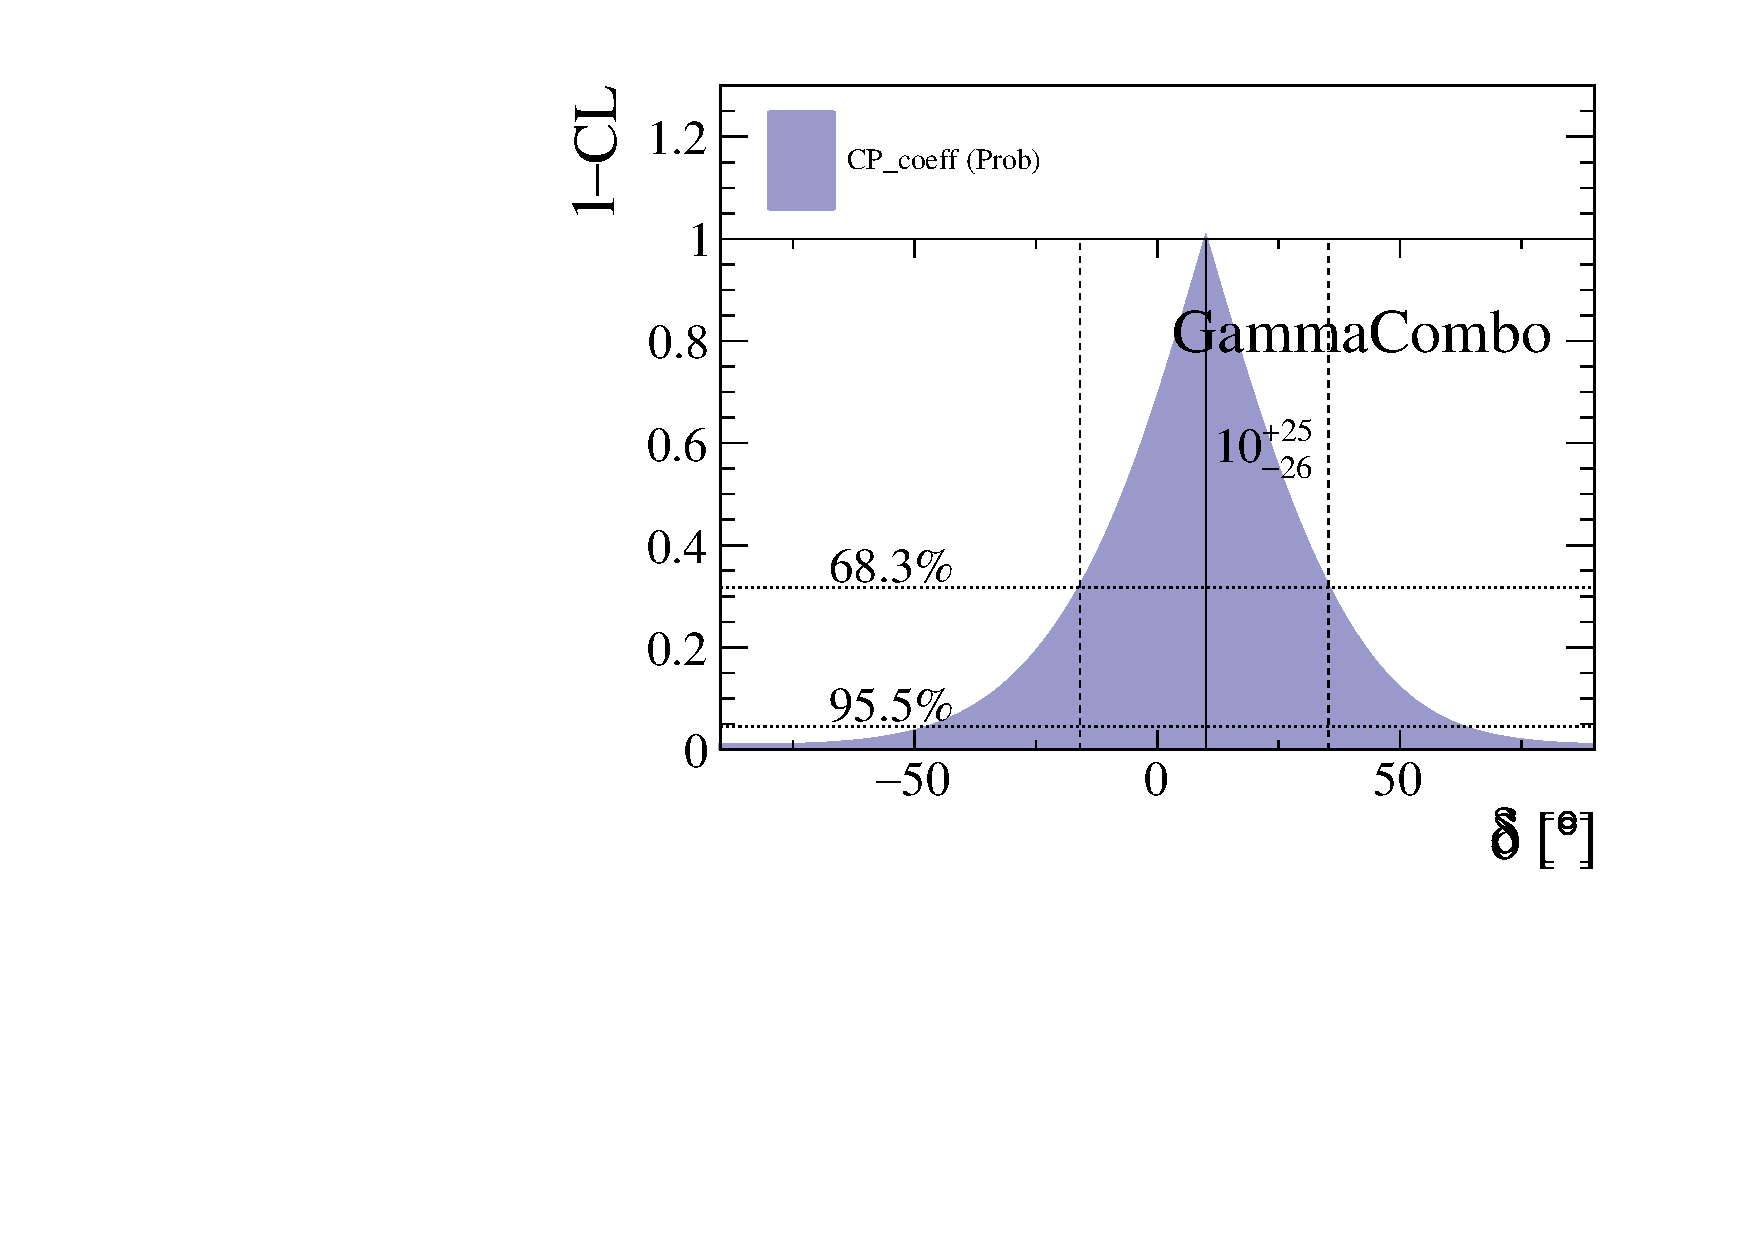
\includegraphics[width=0.4\textwidth, height = !]{figs/GammaCombo/signal_toy/cartesian_cp_coeff_d.pdf} 
		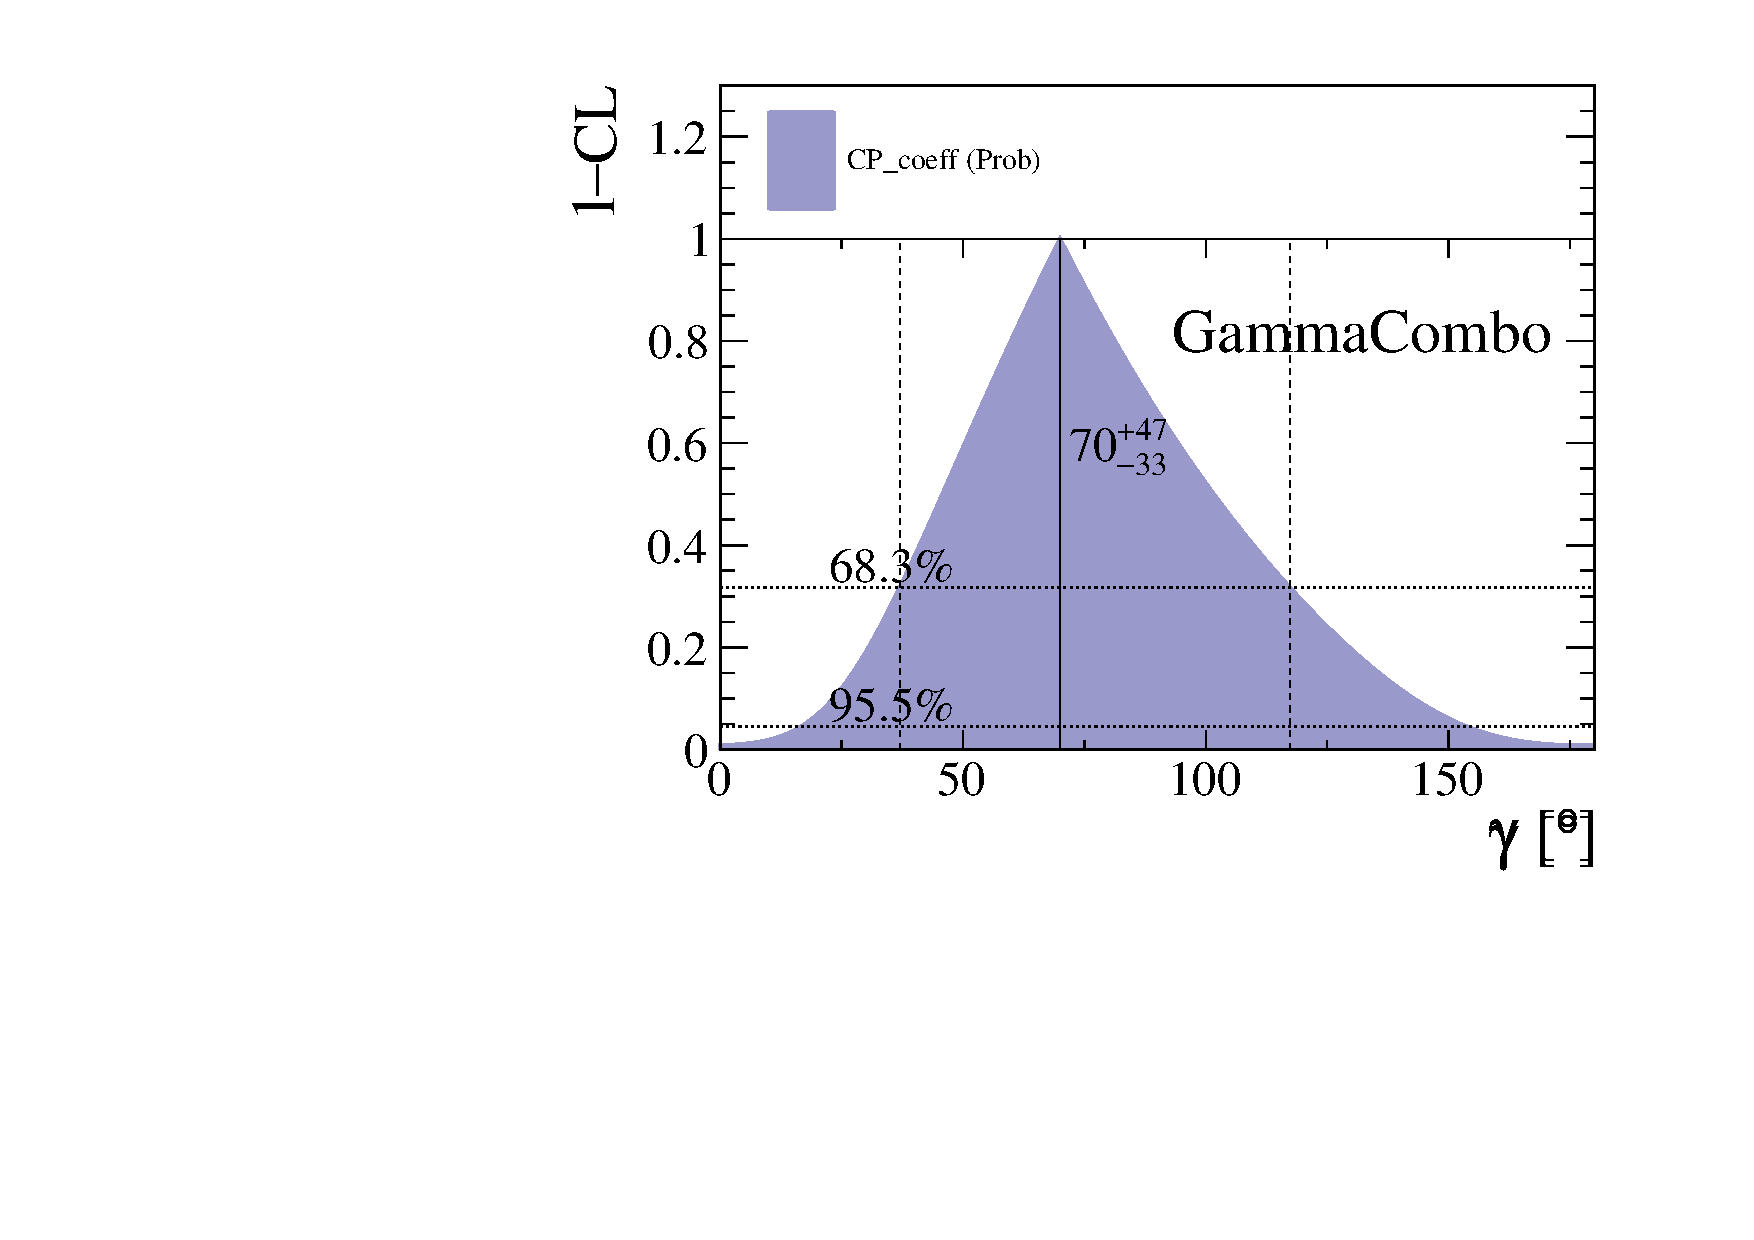
\includegraphics[width=0.4\textwidth, height = !]{figs/GammaCombo/signal_toy/cartesian_cp_coeff_g.pdf} 
		\caption{The 1-CL contours for the physical observable $r,\kappa,\delta$ and $\gamma$ obtained with the phasespace-integrated fit. }
		\label{fig:FitCL}	
\end{figure} 

%\subsection{Determination of $\gamma$ using the measured CP parameters}
%\label{subsec:GammaComb}
%
%The CKM angle $\gamma$, as well as $r$, $\delta$ and $\kappa$ are determined from the measured CP-violating parameters using the \textsf{GammaCombo} package~\cite{GammaCombo}.
%For this, the likelihood 
%
%\begin{equation}
%\mathcal{L}(\alpha) = \exp\left(-\frac{1}{2}(\vec{A}(\vec{\alpha})- \vec{A}_{obs})^{T} V^{-1} (\vec{A}(\vec{\alpha}) - \vec{A}_{obs} ) \right),
%\label{eq:GammaComb}
%\end{equation}
%
%where $\alpha = (\gamma, \beta_{s}, r, \delta)$ is the vector of the physical observables, $\vec{A}$ is the vector of CP-violating observables defined in Equation~\ref{eq:CPcoeff},  
%is the vector of the measured CP parameters given in Table~\ref{tab:sigFitResults} and $V$ is the covariance matrix combining statistics and systematics.
%Following a frequentest approach~\cite{LHCb-PAPER-2013-020}, confidence intervals are given by evaluating the test statistics $\Delta \chi^{2} = \chi^{2}(\vec{\alpha^{'}}_{min}) - \chi^{2}(\vec{\alpha}_{min})$,
%where $\chi^{2}(\vec{\alpha}) = -2 \ln\mathcal{L}(\vec{alpha})$ and $\vec{\alpha}_{min}$ denotes the global maximum of Equation \ref{eq:GammaComb}, 
%while $\vec{alpha^{'}}_{min}$ is the conditional maximum when the parameter of interest is fixed.




%\subsection{\textsf{sFit} model validation using toy studies}
%The fit model and procedure is validated using pseudo experiments. 1000 toys are generated using the model described in Eq. \ref{eq:TPDF_full} and \ref{eq:PDF_intX}. 
%Each pseudo experiment is generated with the same amount of signal events found in the Run I + 2015/2016 data samples.  
%Figure \ref{fig:ToyPulls_tdfit} shows the pull distributions for all CP coefficients, where every pull P of a parameter x is given as $P = \frac{x_{gen} - x_{fit}}{\Delta x}$.
%
%
%\begin{figure}[h]
%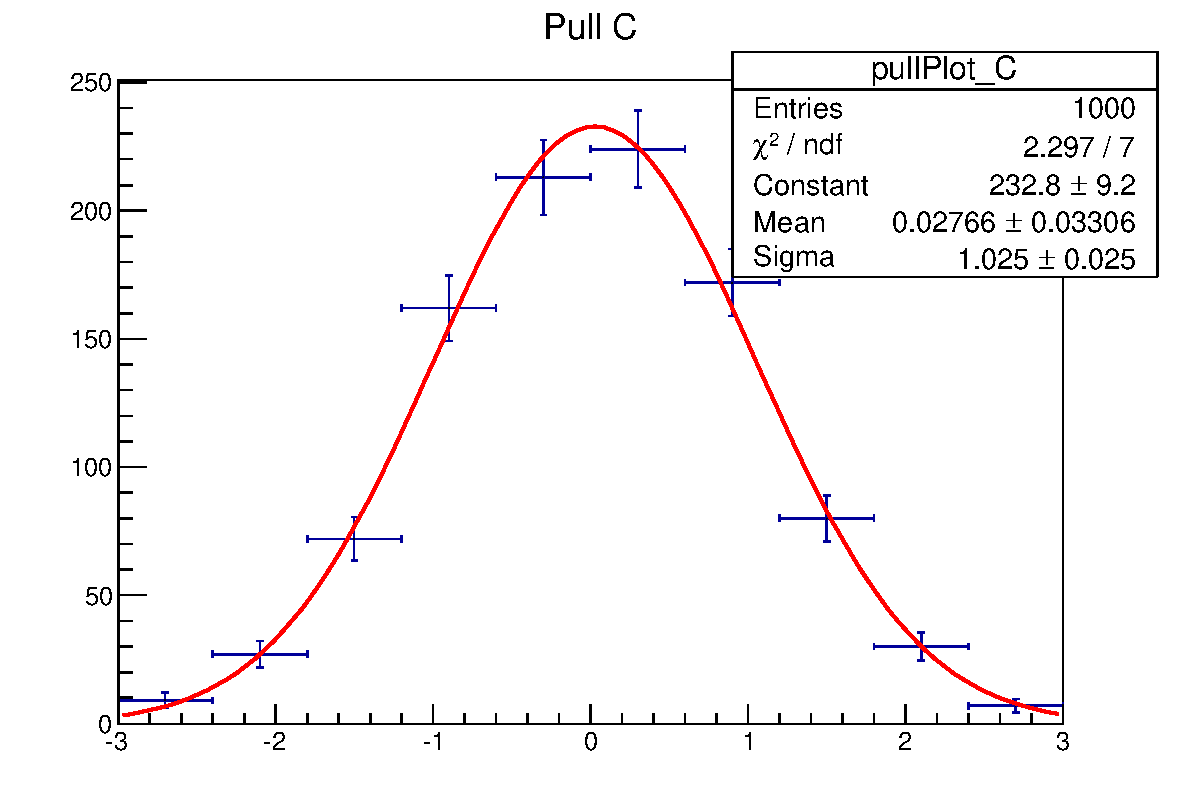
\includegraphics[height=!,width=0.49\textwidth]{figs/plots_toy/studies_timeFit/pull_C_all_Gaussfit.pdf}
%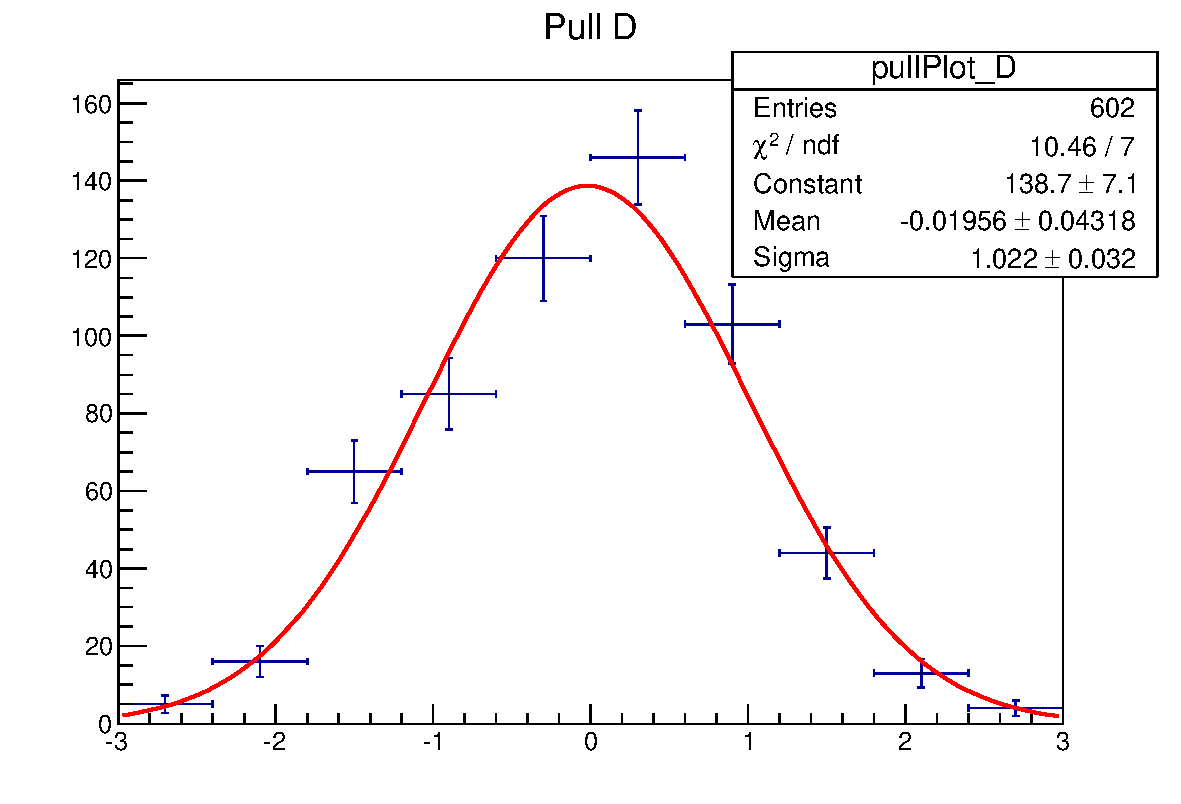
\includegraphics[height=!,width=0.49\textwidth]{figs/plots_toy/studies_timeFit/pull_D_all_Gaussfit.pdf}
%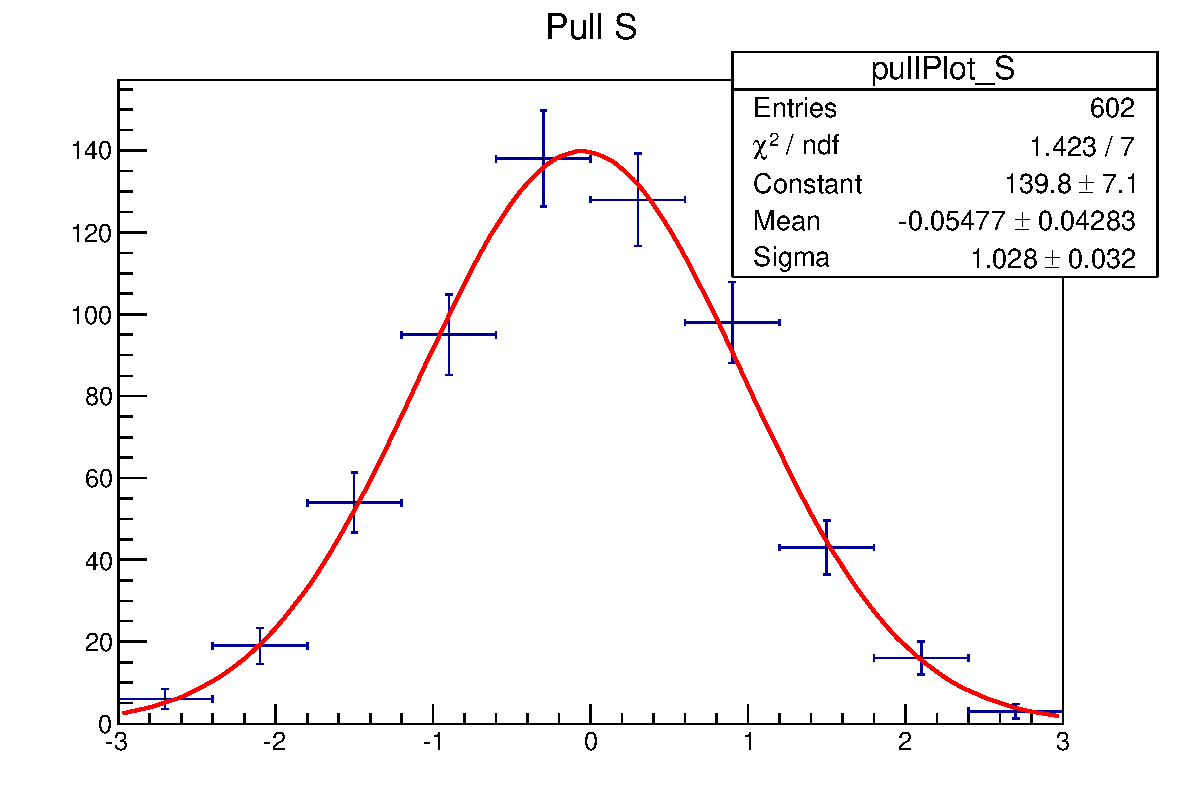
\includegraphics[height=!,width=0.49\textwidth]{figs/plots_toy/studies_timeFit/pull_S_all_Gaussfit.pdf}
%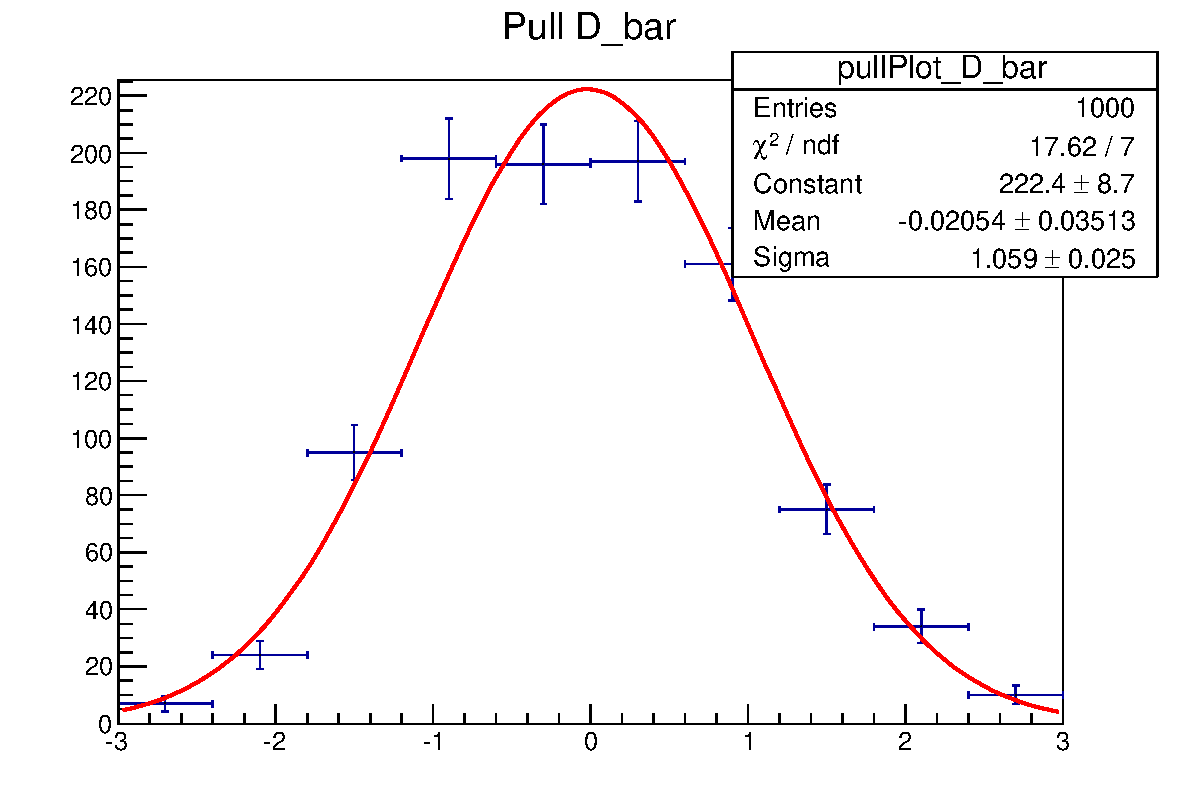
\includegraphics[height=!,width=0.49\textwidth]{figs/plots_toy/studies_timeFit/pull_D_bar_all_Gaussfit.pdf}
%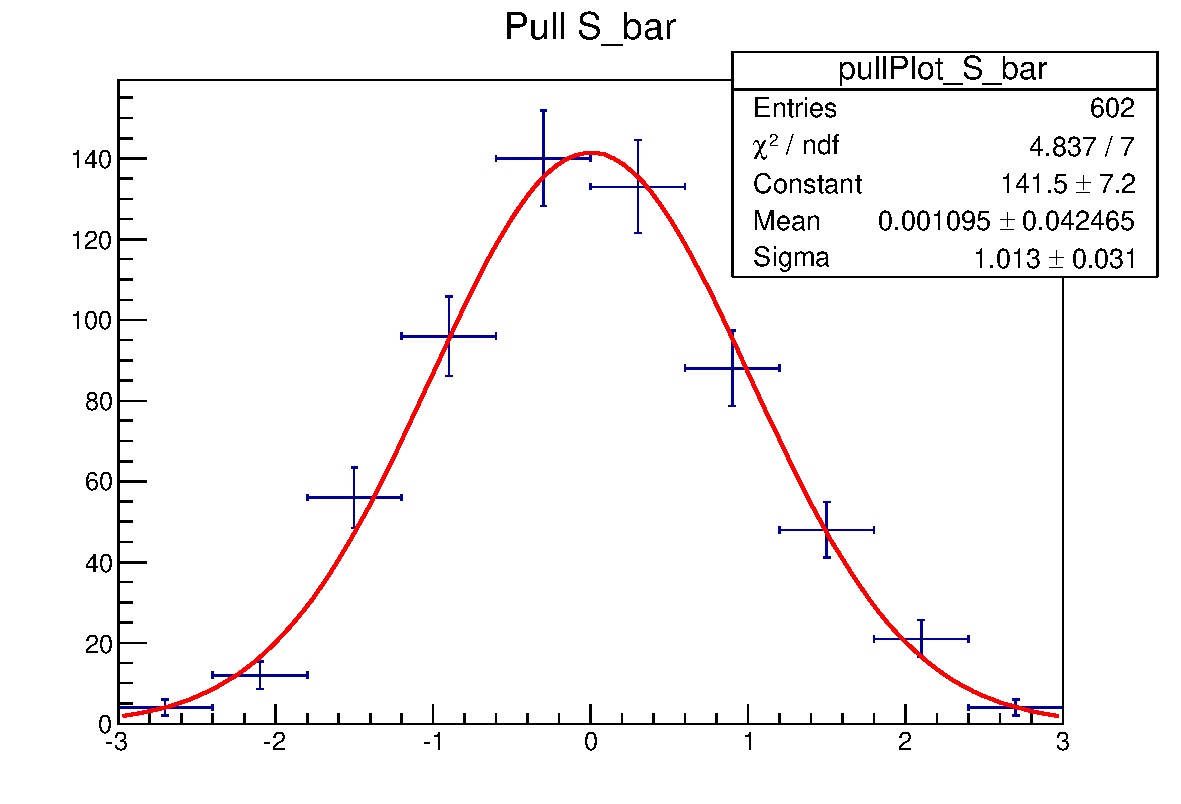
\includegraphics[height=!,width=0.49\textwidth]{figs/plots_toy/studies_timeFit/pull_S_bar_all_Gaussfit.pdf}
%\caption{Pull distributions from toy studies for the time-dependent fit, done with 1000 pseudo experiments.}
%\label{fig:ToyPulls_tdfit}
%\end{figure}
%
%
%\begin{table}[hp!]
\centering
\caption{Pull parameters for CP coefficients from the toy studies for the time-dependent fit.}
\begin{tabular}{l | c | c}
\hline
Parameter & $\mu$ of pull distribution & $\sigma$ of pull distribution \\
\hline
\hline
C & 0.0344147 $\pm$ 0.0424816 & 1.01956 $\pm$ 0.033269 \\
D & -0.0195562 $\pm$ 0.0431762 & 1.0218 $\pm$ 0.031551 \\
S & -0.0547728 $\pm$ 0.0428276 & 1.02791 $\pm$ 0.0318385 \\
$\bar{D}$ & -0.0173495 $\pm$ 0.0469972 & 1.09866 $\pm$ 0.035404 \\
$\bar{S}$ & 0.00109528 $\pm$ 0.0424655 & 1.01306 $\pm$ 0.0313123 \\
\hline
\end{tabular}
\label{table:Pulls_tDFit}
\end{table}
%
%
%Table \ref{table:Pulls_tDFit} summarizes the means $\mu$ and widths $\sigma$ of these pull distributions.

